%*************************************
% บทที่ 3
%*************************************
\chapterTitle{3}{วิธีการดำเนินงาน}

\hspace*{1.3em} %ย่อหน้า
ในการจัดทำโครงงานระบบ เว็บแอปพลิเคชันเพื่อการคอนฟิกด้วยวิธี NETCONF ผ่าน LLM  ฉบับนี้ ผู้จัดทำได้เลือกใช้เทคโนโลยีสมัยใหม่และเครื่องมือที่เหมาะสมสำหรับการพัฒนาระบบจัดการเครือข่ายอัตโนมัติที่ขับเคลื่อนด้วย LLM ซึ่งช่วยให้การพัฒนาระบบที่มีความซับซ้อนเป็นไปได้อย่างมีประสิทธิภาพและตามมาตรฐานสากล รายละเอียดของวิธีการดำเนินงาน มีดังต่อไปนี้
\section{การเตรียมสภาพแวดล้อมการพัฒนา}

\hspace*{1.3em} %ย่อหน้า
ก่อนเริ่มต้นการพัฒนาระบบ ผู้จัดทำได้ดำเนินการเตรียมความพร้อมของสภาพแวดล้อมที่จำเป็นสำหรับการพัฒนา Full-Stack Application ดังนี้

\begin{mycustomenum2}
    \item \textbf{การติดตั้งเครื่องมือพัฒนาหลัก}
    \begin{mycustomenum2}
        \item \textbf{Node.js (v18+):} JavaScript runtime สำหรับการพัฒนา backend และ frontend
        \item \textbf{MongoDB Atlas:} Cloud database service สำหรับจัดเก็บข้อมูลอุปกรณ์เครือข่ายและประวัติการคอนฟิก
        \item \textbf{Ollama:} Local LLM inference server สำหรับ LLM models
        \item \textbf{Git} Version control system สำหรับการจัดการโค้ดต้นฉบับ
    \end{mycustomenum2}
    \item \textbf{โปรแกรมเขียนโค้ดและแก้ไขโค้ด}
    \begin{mycustomenum2}
        \item \textbf{Cursor IDE:} เป็น AI-powered code editor ที่มีฟังก์ชันการเขียนโค้ดแบบอัจฉริยะ การแนะนำโค้ด และการตรวจสอบข้อผิดพลาดแบบ real-time พร้อมรองรับการทำงานกับ multiple languages (JavaScript, JSX, CSS)
        \item \textbf{Visual Studio Code:} เป็น lightweight code editor ที่มี extension ecosystem ที่หลากหลาย เหมาะสำหรับการพัฒนา web application และการจัดการ Git integration
    \end{mycustomenum2}
\end{mycustomenum2}

\hspace*{1.3em} %ย่อหน้า

\hspace*{1.3em} %ย่อหน้า

\hspace*{1.3em} %ย่อหน้า

\hspace*{1.3em} %ย่อหน้า

\section{สถาปัตยกรรมระบบและเทคโนโลยีที่ใช้}

\hspace*{1.3em} %ย่อหน้า
ระบบได้รับการออกแบบด้วย Modern Full-Stack Architecture โดยแยกเป็นส่วนต่าง ๆ ดังนี้

\subsection{Backend Development (Server-side)}
\begin{mycustomitem2}
    \item \textbf{Framework:} Express.js สำหรับการสร้าง RESTful API
    \item \textbf{Deployment:} Vercel Serverless Functions สำหรับ Deploy backend แบบ Serverless
    \item \textbf{Database:} MongoDB Atlas พร้อม Mongoose ODM สำหรับจัดการข้อมูล
    \item \textbf{Authentication:} Google OAuth 2.0 สำหรับการยืนยันตัวตนผู้ใช้
    \item \textbf{Agent Relay:} ระบบ Command Queue ผ่าน MongoDB เพื่อสื่อสารกับ Desktop Agent แบบ HTTP Polling (Long-polling สูงสุด 55 วินาที พร้อม Extended Polling สำหรับ Restore)
\end{mycustomitem2}

\subsection{Frontend Development (Client-side)}
\begin{mycustomitem2}
    \item \textbf{Framework:} React 19 ร่วมกับ Vite 6 build tool
    \item \textbf{UI Framework:} Tailwind CSS สำหรับการออกแบบ responsive interface
    \item \textbf{State Management:} React Hooks และ Context API
    \item \textbf{HTTP Client:} Axios สำหรับการสื่อสารกับ backend
    \item \textbf{Analytics:} Vercel Speed Insights สำหรับวัดประสิทธิภาพ
\end{mycustomitem2}

\subsection{Desktop Agent (Electron Application)}
\begin{mycustomitem2}
    \item \textbf{Framework:} Electron สำหรับสร้าง Desktop Application ที่รันบนเครื่องผู้ใช้
    \item \textbf{Communication:} HTTP Polling ทุก 2 วินาทีเพื่อรับคำสั่งจาก Backend ผ่าน Agent Relay (Long-polling สูงสุด 55 วินาที)
    \item \textbf{Network Protocols:} SSH2 สำหรับเชื่อมต่อกับอุปกรณ์เครือข่าย (รองรับ Interactive Shell สำหรับ Backup), NETCONF over SSH (Port 830) พร้อม Auto-Connect
    \item \textbf{LLM Integration:} Ollama API สำหรับเชื่อมต่อกับ LLM models ที่รันบนเครื่องผู้ใช้ (qwen2.5-coder:7b)
    \item \textbf{Serial Console:} SerialPort สำหรับเชื่อมต่ออุปกรณ์ผ่าน Console Port พร้อมแสดง Port ทุกประเภท (USB-to-Serial, Bluetooth, Serial) โดยไม่กรองออก
    \item \textbf{Console Relay:} ระบบตรวจจับ SerialPort availability (\textbf{serialPortAvailable} flag) เพื่อ Relay คำสั่ง Console ไปยัง Desktop Agent อัตโนมัติบน Vercel Serverless ที่ไม่สามารถใช้ Native Module ได้
    \item \textbf{NETCONF Auto-Connect:} ระบบเชื่อมต่อ NETCONF อัตโนมัติเมื่อต้องการดำเนินการ (ensureConnected) เพื่อรองรับ Vercel Serverless ที่ไม่มี persistent state
    \item \textbf{Backup Interactive Shell:} ใช้ Interactive Shell แทน Single Exec เพื่อรองรับ Multi-command Sequence บนอุปกรณ์ Cisco
\end{mycustomitem2}

\subsection{Intelligent Services}
\begin{mycustomitem2}
    \item \textbf{Text Generation:} Ollama LLM Service (ผ่าน Desktop Agent) สำหรับการสร้าง configuration จาก natural language prompts
    \item \textbf{Knowledge Base:} Comprehensive Cisco networking knowledge base ที่ embedded ในระบบ
\end{mycustomitem2}


\section{System Overview Diagram}

\begin{figure}[H]
\centering
\adjustbox{width=1.0\textwidth}{%สร้างกรอบของภาพ
    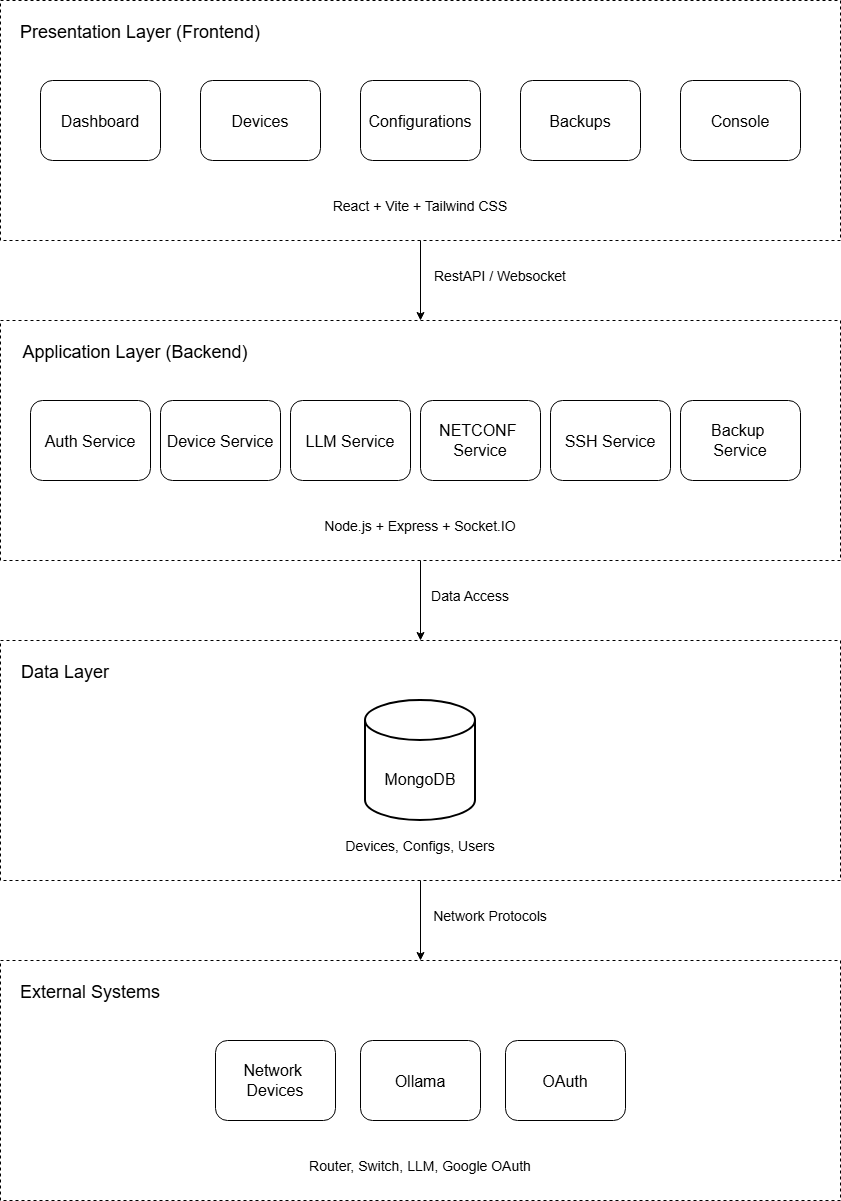
\includegraphics[width=1.0\textwidth]{Image/SOD.png}
}
\caption{\fontSixTeen{แสดงการทำงานและลำดับขั้นตอนโดยรวมของโปรแกรม}}
\label{fig3:OverviewDiagram}
\end{figure}

\section{Context Diagram}

\begin{figure}[H]
\centerline{
    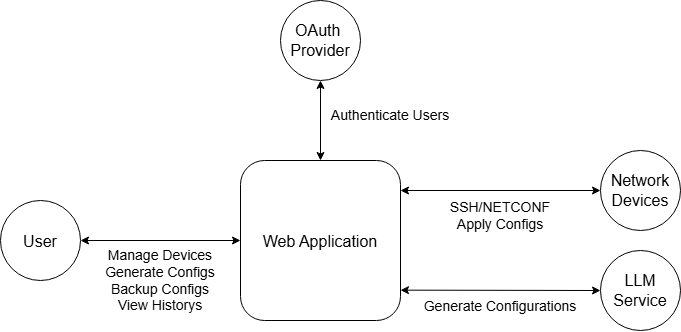
\includegraphics[width=1\textwidth]{Image/CD.png}
}

\caption{\fontSixTeen{Context Diagram}}
\label{fig3:ContextDiagram}
\end{figure}

\hspace*{1.3em} %ย่อหน้า
จากภาพที่ \ref{fig3:ContextDiagram} แสดง Context Diagram ของระบบเว็บแอปพลิเคชันเพื่อการคอนฟิกด้วยวิธี NETCONF ผ่าน LLM ซึ่งแสดง External Entities ทั้งหมดที่มีปฏิสัมพันธ์กับระบบ ดังนี้

\begin{mycustomitem2}
    \item \textbf{Network Admin (ผู้ดูแลระบบเครือข่าย):} ผู้ใช้งานหลักของระบบ สามารถป้อนคำสั่ง Configuration Requests เป็นภาษาธรรมชาติ จัดการอุปกรณ์ (CRUD) สำรองและกู้คืนคอนฟิก เชื่อมต่อ Console ผ่าน SSH และรับผลลัพธ์ต่าง ๆ กลับมา (F1, F2)
    \item \textbf{Google OAuth 2.0:} ระบบยืนยันตัวตนภายนอก ใช้สำหรับ Login ผ่าน OAuth Authorization Request และรับ JWT Token กลับมาเพื่อใช้งานระบบ (F7, F8)
    \item \textbf{Ollama LLM API:} ระบบ AI สำหรับสร้าง Configuration โดยรับ AI Prompt พร้อมประเภทอุปกรณ์ (NX-OS/IOS-XE) และ YANG Templates แล้วส่งคืน Generated CLI/NETCONF XML Configuration (F5, F6)
    \item \textbf{Desktop Agent (Electron App):} แอปพลิเคชันที่รันบนเครื่องผู้ใช้ ทำหน้าที่เป็นตัวกลาง (Agent Relay) ระหว่าง Backend กับอุปกรณ์เครือข่าย โดยรับคำสั่ง SSH/NETCONF, Backup Requests และ Console Port Scan ผ่าน HTTP Polling แล้วส่งผลลัพธ์กลับ ได้แก่ การเชื่อมต่อ SSH, การ Deploy Config, การสำรองข้อมูล รวมถึงการเชื่อมต่อ Serial Console (F11-F14)
    \item \textbf{Network Devices (อุปกรณ์เครือข่าย):} อุปกรณ์ Cisco NX-OS และ IOS-XE ที่ระบบสื่อสารผ่าน SSH/NETCONF โดยผ่าน Desktop Agent เพื่อส่ง CLI Commands และ NETCONF/YANG XML แล้วรับ Running Config และ Device Capabilities กลับมา (F3, F4)
    \item \textbf{MongoDB Atlas:} ฐานข้อมูลกลางของระบบ (9 Collections: D1-D9) สำหรับจัดเก็บข้อมูลผู้ใช้ อุปกรณ์ ประวัติคอนฟิก สำรองข้อมูล YANG Models คำสั่ง Agent Heartbeat Notifications และ Shell Sessions (F9, F10)
\end{mycustomitem2}

\section{Dataflow Diagram (DFD)}

\begin{figure}[H]
    \centering
    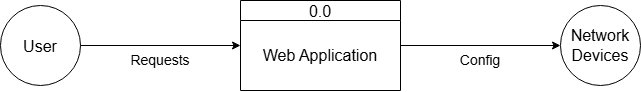
\includegraphics[width=\textwidth]{Image/Level-0.png}
    \caption{\fontSixTeen{DFD ระดับที่ 1 กระบวนการหลักของระบบ (Main Process Decomposition)}}
\label{fig3:DataflowDiagram}
\end{figure}

\hspace*{1.3em} %ย่อหน้า
จากภาพที่ \ref{fig3:DataflowDiagram} แสดง DFD ระดับที่ 1 ซึ่งแบ่งระบบออกเป็น 6 กระบวนการหลัก ดังนี้

\begin{mycustomitem2}
    \item \textbf{Process 1.0 Authentication:} ตรวจสอบตัวตนผู้ใช้ผ่าน Google OAuth 2.0 ออก JWT Token และจัดการ Session
    \item \textbf{Process 2.0 Device Management:} จัดการอุปกรณ์เครือข่าย (เพิ่ม แก้ไข ลบ) รองรับประเภท Router, Switch, Nexus (NX-OS) และ IOS-XE พร้อมทดสอบการเชื่อมต่อ SSH/NETCONF ผ่าน Desktop Agent
    \item \textbf{Process 3.0 Configuration Generation:} สร้าง Configuration อัตโนมัติด้วย AI (Ollama LLM) ที่รันบนเครื่องผู้ใช้ โดยเชื่อมต่อผ่าน Agent Relay $\rightarrow$ Desktop Agent $\rightarrow$ Ollama (Local) รับ Prompt ภาษาธรรมชาติ แล้วสร้าง CLI หรือ NETCONF/YANG XML สำหรับอุปกรณ์ NX-OS System และ IOS-XE native
    \item \textbf{Process 4.0 Deployment:} ติดตั้ง Configuration ไปยังอุปกรณ์เครือข่ายผ่าน Agent Relay $\rightarrow$ Desktop Agent $\rightarrow$ SSH (CLI) หรือ NETCONF/YANG พร้อมติดตามสถานะการ Deploy
    \item \textbf{Process 5.0 Backup Management:} สำรองและกู้คืน Configuration ผ่าน Agent Relay $\rightarrow$ Desktop Agent $\rightarrow$ SSH (Interactive Shell) พร้อมตรวจสอบความซ้ำด้วย SHA-256 Hash
    \item \textbf{Process 6.0 Console Management:} จัดการ Interactive SSH Shell ผ่าน Agent Relay $\rightarrow$ Desktop Agent แบบ Polling-based I/O Buffer สำหรับเชื่อมต่อ Terminal กับอุปกรณ์
\end{mycustomitem2}

\hspace*{1.3em} %ย่อหน้า
ระบบมี Data Store ทั้งหมด 7 ตาราง ได้แก่ D1 Users, D2 Devices, D3 Configs, D4 Backups, D5 YANG Models, D6 Agent Commands และ D7 Shell Sessions โดยมี External Entities ได้แก่ ผู้ใช้ (Network Admin), Google OAuth, Desktop Agent, Ollama LLM (Local, เข้าถึงผ่าน Desktop Agent) และอุปกรณ์เครือข่าย

\begin{figure}[H]
    \centerline{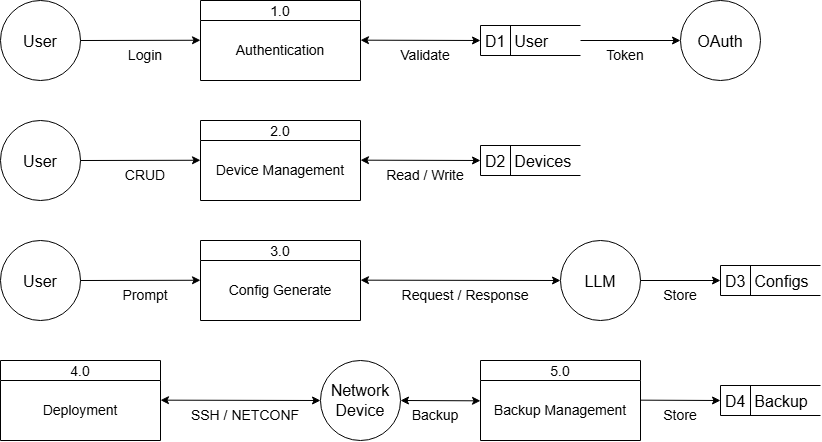
\includegraphics[width=\textwidth]{Image/Level-1.png}}
    \caption{\fontSixTeen{DFD ระดับที่ 2 ของ Process 2.0 (Device Management)}}
    \label{fig3:DataflowDiagram_Level2_Process2.0}
\end{figure}

\hspace*{1.3em} %ย่อหน้า
จากภาพที่ \ref{fig3:DataflowDiagram_Level2_Process2.0} แสดงการแยกย่อย Process 2.0 Device Management ออกเป็น 5 กระบวนการย่อย ได้แก่ 2.1 เพิ่มอุปกรณ์ 2.2 แก้ไขอุปกรณ์ 2.3 ลบอุปกรณ์ 2.4 ทดสอบการเชื่อมต่อ (SSH/NETCONF ผ่าน Desktop Agent) และ 2.5 แสดงรายการอุปกรณ์ทั้งหมด โดยเชื่อมต่อกับ D1 ฐานข้อมูลอุปกรณ์ และอุปกรณ์เครือข่ายจริง

\begin{figure}[H]
    \centerline{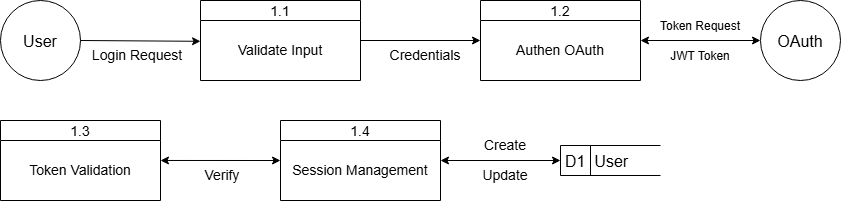
\includegraphics[width=1.0\textwidth]{Image/Level-2.png}}
    \caption{\fontSixTeen{DFD ระดับที่ 2 ของ Process 3.0 (Configuration Generation)}}
    \label{fig3:DataflowDiagram_Level2_Process3.0}
\end{figure}

\hspace*{1.3em} %ย่อหน้า
จากภาพที่ \ref{fig3:DataflowDiagram_Level2_Process3.0} แสดงการแยกย่อย Process 3.0 Configuration Generation ออกเป็น 5 กระบวนการย่อย ได้แก่ 3.1 รับ Prompt จากผู้ใช้ 3.2 เตรียมบริบท (โหลดข้อมูลอุปกรณ์และตรวจจับประเภท NX-OS/IOS-XE) 3.3 เรียกใช้ Ollama LLM ผ่าน Agent Relay $\rightarrow$ Desktop Agent $\rightarrow$ Ollama (Local) เพื่อสร้าง CLI หรือ NETCONF/YANG XML 3.4 ตรวจสอบ Syntax และ Namespace ของคอนฟิกที่สร้าง และ 3.5 บันทึกคอนฟิกและ Explanation ลงฐานข้อมูลประวัติ

\begin{figure}[H]
    \centerline{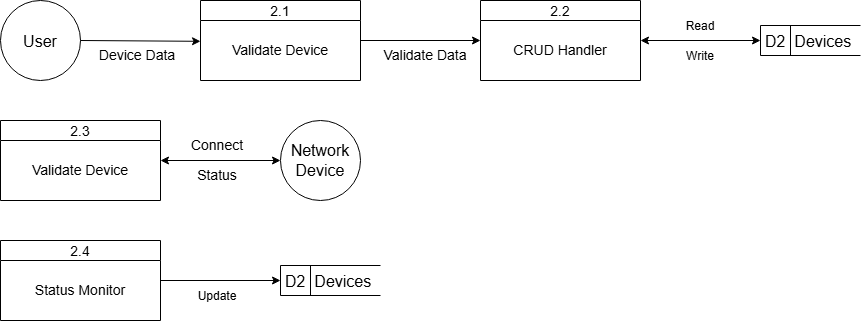
\includegraphics[width=1.0\textwidth]{Image/Level-3.png}}
    \caption{\fontSixTeen{DFD ระดับที่ 2 ของ Process 4.0 (Configuration Deployment)}}
    \label{fig3:DataflowDiagram_Level2_Process4.0}
\end{figure}

\hspace*{1.3em} %ย่อหน้า
จากภาพที่ \ref{fig3:DataflowDiagram_Level2_Process4.0} แสดงการแยกย่อย Process 4.0 Configuration Deployment ออกเป็น 4 กระบวนการย่อย ได้แก่ 4.1 เลือกคอนฟิก (CLI/NETCONF) ที่ต้องการ Deploy 4.2 โหลดข้อมูลอุปกรณ์และตรวจจับประเภท 4.3 Deploy คอนฟิกผ่าน Agent Relay $\rightarrow$ Desktop Agent $\rightarrow$ SSH (CLI) หรือ NETCONF/YANG และ 4.4 อัปเดตสถานะการ Deploy และบันทึกประวัติ

\begin{figure}[H]
    \centerline{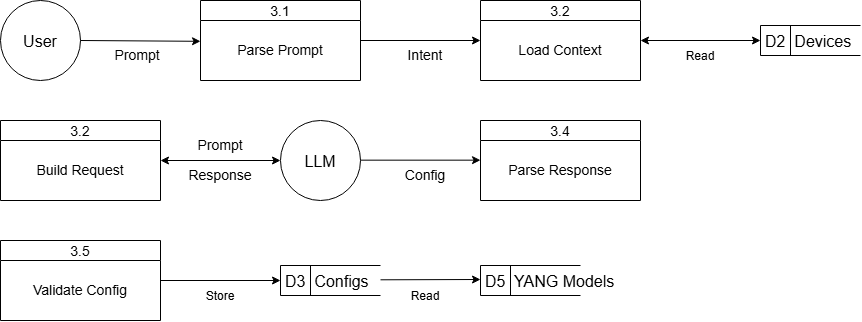
\includegraphics[width=1.0\textwidth]{Image/Level-4.png}}
    \caption{\fontSixTeen{DFD ระดับที่ 2 ของ Process 5.0 (Backup Management)}}
    \label{fig3:DataflowDiagram_Level2_Process5.0}
\end{figure}

\hspace*{1.3em} %ย่อหน้า
จากภาพที่ \ref{fig3:DataflowDiagram_Level2_Process5.0} แสดงการแยกย่อย Process 5.0 Backup Management ออกเป็น 4 กระบวนการย่อย ได้แก่ 5.1 เริ่ม Backup (โหลดข้อมูลอุปกรณ์) 5.2 ดึงคอนฟิกจากอุปกรณ์ผ่าน Agent Relay $\rightarrow$ Desktop Agent $\rightarrow$ SSH (show running-config) 5.3 ตรวจสอบความซ้ำด้วย SHA-256 Hash และ 5.4 บันทึก Backup พร้อม Metadata, Tags และ Timestamp นอกจากนี้ยังรองรับ Auto Trigger จาก Scheduler สำหรับ Backup อัตโนมัติ

\begin{figure}[H]
    \centerline{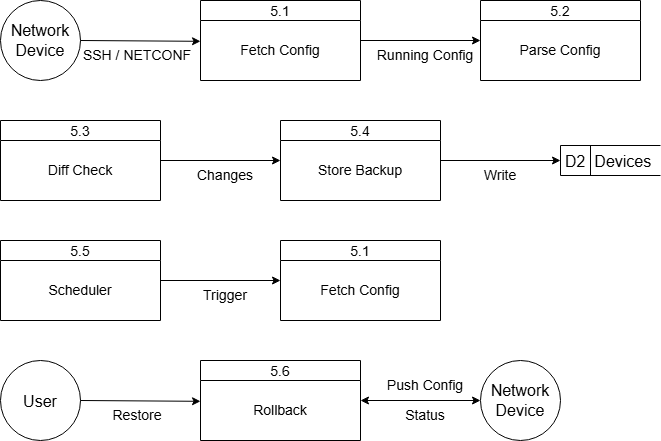
\includegraphics[width=1.0\textwidth]{Image/Level-5.png}}
    \caption{\fontSixTeen{DFD ระดับที่ 2 ของ Process 6.0 (Console Management)}}
    \label{fig3:DataflowDiagram_Level2_Process6.0}
\end{figure}

\hspace*{1.3em} %ย่อหน้า
จากภาพที่ \ref{fig3:DataflowDiagram_Level2_Process6.0} แสดงการแยกย่อย Process 6.0 Console Management ออกเป็น 5 กระบวนการย่อย ได้แก่ 6.1 สแกน Serial Port ที่พร้อมใช้งาน (COM/USB) ผ่าน Desktop Agent 6.2 เชื่อมต่อ Console ด้วยการตั้งค่า Baud Rate, Data Bits และ Parity ผ่าน Agent Relay $\rightarrow$ Desktop Agent 6.3 ส่งคำสั่ง CLI ไปยังอุปกรณ์ผ่าน Serial Console 6.4 Push Initial Configuration (Hostname, IP, Credentials) ไปยังอุปกรณ์ใหม่ และ 6.5 ปิดการเชื่อมต่อ Serial Port และอัปเดตสถานะ Session

\section{พจนานุกรมข้อมูล (Data Flow Description)}

% =====================================================
% DF-6: Serial Console Configuration
% =====================================================

\begin{table}[H]
    \caption{\fontSixTeen{แสดง Data Flow การเชื่อมต่อ Serial Console}}
    \label{tab:df-6-1}
    \fontSixTeen 
    \begin{tabularx}{\textwidth}{|l|L|} 
        \hline
        \textbf{Data Flow ID:} & DF-6.1 \\
        \hline
        \textbf{Data Flow Name:} & การเชื่อมต่อ Serial Console \\
        \hline
        \textbf{Description:} & กระบวนการที่ผู้ใช้ทำการเชื่อมต่อกับอุปกรณ์เครือข่ายผ่าน Serial Port เพื่อคอนฟิกเริ่มต้นและเปิดใช้งาน SSH \\
        \hline
        \textbf{Source:} & ผู้ใช้ (User) \\
        \hline
        \textbf{Destination:} & อุปกรณ์เครือข่าย (Network Device) \\
        \hline
        \textbf{Type Of Data Flow:} & Serial Connection \\
        \hline
        \textbf{Data Structure:} & ข้อมูลการเชื่อมต่อ Serial = \{ \nonumber \\
                        & \hspace{1em} ``portPath'' : ``เช่น COM3 หรือ /dev/ttyUSB0'', \nonumber \\
                        & \hspace{1em} ``baudRate'' : ``9600 (default) | 19200 | 38400 | 57600 | 115200'', \nonumber \\
                        & \hspace{1em} ``dataBits'' : ``8 (default)'', \nonumber \\
                        & \hspace{1em} ``parity'' : ``none (default) | odd | even'', \nonumber \\
                        & \hspace{1em} ``stopBits'' : ``1 (default) | 2'', \nonumber \\
                        & \hspace{1em} ``flowControl'' : ``false (default) | true'', \nonumber \\
                        & \hspace{1em} ``deviceId'' : ``รหัสเซสชันของอุปกรณ์ (ObjectId)'' \nonumber \\
                        & \} \\
        \hline
    \end{tabularx}
\end{table}

\begin{table}[H]
    \caption{\fontSixTeen{แสดง Data Flow การคอนฟิก SSH เริ่มต้น}}
    \label{tab:df-6-2}
    \fontSixTeen 
    \begin{tabularx}{\textwidth}{|l|L|} 
        \hline
        \textbf{Data Flow ID:} & DF-6.2 \\
        \hline
        \textbf{Data Flow Name:} & คำสั่งการตั้งค่าเริ่มต้น \\
        \hline
        \textbf{Description:} & ข้อมูลการตั้งค่าเริ่มต้นที่ส่งไปยังอุปกรณ์เครือข่ายผ่าน Serial Console เพื่อเปิดใช้งาน SSH \\
        \hline
        \textbf{Source:} & ผู้ใช้ (User) \\
        \hline
        \textbf{Destination:} & อุปกรณ์เครือข่าย (Network Device) \\
        \hline
        \textbf{Type Of Data Flow:} & Configuration Data \\
        \hline
        \textbf{Data Structure:} & ข้อมูลการตั้งค่าเริ่มต้น = \{ \nonumber \\
                        & \hspace{1em} ``hostname'' : ``ชื่อโฮสต์ของอุปกรณ์'', \nonumber \\
                        & \hspace{1em} ``interface'' : ``ชื่ออินเทอร์เฟซ เช่น GigabitEthernet0/1'', \nonumber \\
                        & \hspace{1em} ``managementIp'' : ``IP Address ของอุปกรณ์'', \nonumber \\
                        & \hspace{1em} ``managementMask'' : ``Subnet Mask'', \nonumber \\
                        & \hspace{1em} ``defaultGateway'' : ``Default Gateway IP'', \nonumber \\
                        & \hspace{1em} ``domain'' : ``ชื่อโดเมนของอุปกรณ์'', \nonumber \\
                        & \hspace{1em} ``username'' : ``ชื่อผู้ใช้สำหรับ SSH'', \nonumber \\
                        & \hspace{1em} ``password'' : ``รหัสผ่านสำหรับ SSH'', \nonumber \\
                        & \hspace{1em} ``rsaKeySize'' : ``ขนาด RSA Key (default: 2048)'' \nonumber \\
                        & \} \\
        \hline
    \end{tabularx}
\end{table}

% =====================================================
% DF-1: Device Management
% =====================================================

\begin{table}[H]
    \caption{\fontSixTeen{แสดง Data Flow ข้อมูลอุปกรณ์}}
    \label{tab:df-1-1}
    \fontSixTeen 
    \begin{tabularx}{\textwidth}{|l|L|} 
        \hline
        \textbf{Data Flow ID:} & DF-1.1 \\
        \hline
        \textbf{Data Flow Name:} & ข้อมูลอุปกรณ์ \\
        \hline
        \textbf{Description:} & ข้อมูลของอุปกรณ์เครือข่ายที่ผู้ใช้บันทึกเข้าสู่ระบบเพื่อการจัดการ \\
        \hline
        \textbf{Source:} & ผู้ใช้ (User) \\
        \hline
        \textbf{Destination:} & D1 ฐานข้อมูลอุปกรณ์ (Device Database) \\
        \hline
        \textbf{Type Of Data Flow:} & Device Data \\
        \hline
        \textbf{Data Structure:} & ข้อมูลอุปกรณ์ = \{ \nonumber \\
                        & \hspace{1em} ``name'' : ``ชื่ออุปกรณ์ เช่น Core-Switch-01 (สูงสุด 255 ตัวอักษร)'', \nonumber \\
                        & \hspace{1em} ``type'' : ``router | switch | nexus | ios-xe'', \nonumber \\
                        & \hspace{1em} ``layer'' : ``layer-2 | layer-3 (เฉพาะ switch)'', \nonumber \\
                        & \hspace{1em} ``ip\_address'' : ``IP Address เช่น 192.168.1.10'', \nonumber \\
                        & \hspace{1em} ``ssh\_port'' : ``พอร์ต SSH (default: 22, range: 1-65535)'', \nonumber \\
                        & \hspace{1em} ``netconf\_port'' : ``พอร์ต NETCONF (default: 830)'', \nonumber \\
                        & \hspace{1em} ``netconf\_enabled'' : ``true | false (default: true สำหรับ nexus และ ios-xe)'', \nonumber \\
                        & \hspace{1em} ``username'' : ``ชื่อผู้ใช้สำหรับ SSH (สูงสุด 255 ตัวอักษร)'', \nonumber \\
                        & \hspace{1em} ``password'' : ``รหัสผ่านสำหรับ SSH'', \nonumber \\
                        & \hspace{1em} ``enable\_password'' : ``รหัสผ่าน Enable (Optional)'', \nonumber \\
                        & \hspace{1em} ``description'' : ``คำอธิบายอุปกรณ์'', \nonumber \\
                        & \hspace{1em} ``location'' : ``ตำแหน่งที่ตั้ง เช่น Data Center Rack A1'', \nonumber \\
                        & \hspace{1em} ``model'' : ``รุ่นของอุปกรณ์ เช่น Cisco ISR 4321'', \nonumber \\
                        & \hspace{1em} ``vendor'' : ``cisco | juniper | huawei | arista | other'', \nonumber \\
                        & \hspace{1em} ``status'' : ``active | inactive | maintenance | error'' \nonumber \\
                        & \} \\
        \hline
    \end{tabularx}
\end{table}

\begin{table}[H]
    \caption{\fontSixTeen{แสดง Data Flow การทดสอบการเชื่อมต่อ}}
    \label{tab:df-1-2}
    \fontSixTeen 
    \begin{tabularx}{\textwidth}{|l|L|} 
        \hline
        \textbf{Data Flow ID:} & DF-1.2 \\
        \hline
        \textbf{Data Flow Name:} & การทดสอบการเชื่อมต่อ \\
        \hline
        \textbf{Description:} & กระบวนการทดสอบการเชื่อมต่อกับอุปกรณ์เครือข่ายผ่าน Agent Relay $\rightarrow$ Desktop Agent $\rightarrow$ SSH \\
        \hline
        \textbf{Source:} & กระบวนการจัดการอุปกรณ์ (Device Management Process) \\
        \hline
        \textbf{Destination:} & Desktop Agent $\rightarrow$ อุปกรณ์เครือข่าย (Network Device) \\
        \hline
        \textbf{Type Of Data Flow:} & Test Connection (via Agent Relay) \\
        \hline
        \textbf{Data Structure:} & ผลการทดสอบ = \{ \nonumber \\
                        & \hspace{1em} ``device\_id'' : ``รหัสอุปกรณ์ (ObjectId)'', \nonumber \\
                        & \hspace{1em} ``ssh\_status'' : ``connected | disconnected | connecting | error'', \nonumber \\
                        & \hspace{1em} ``ssh\_connected\_at'' : ``เวลาที่เชื่อมต่อ (Date)'', \nonumber \\
                        & \hspace{1em} ``ssh\_session\_id'' : ``รหัสเซสชัน SSH'', \nonumber \\
                        & \hspace{1em} ``last\_connection'' : \{ \nonumber \\
                        & \hspace{2em} ``type'' : ``ssh | console'', \nonumber \\
                        & \hspace{2em} ``timestamp'' : ``เวลาที่เชื่อมต่อ'', \nonumber \\
                        & \hspace{2em} ``status'' : ``success | failed | timeout'', \nonumber \\
                        & \hspace{2em} ``error\_message'' : ``ข้อความผิดพลาด (ถ้ามี)'' \nonumber \\
                        & \hspace{1em} \} \nonumber \\
                        & \} \\
        \hline
    \end{tabularx}
\end{table}

% =====================================================
% DF-2: Configuration Generation
% =====================================================

\begin{table}[H]
    \caption{\fontSixTeen{แสดง Data Flow คำขอสร้างคอนฟิก}}
    \label{tab:df-2-1}
    \fontSixTeen 
    \begin{tabularx}{\textwidth}{|l|L|} 
        \hline
        \textbf{Data Flow ID:} & DF-2.1 \\
        \hline
        \textbf{Data Flow Name:} & คำขอสร้างคอนฟิก \\
        \hline
        \textbf{Description:} & คำสั่งหรือข้อความ Prompt จากผู้ใช้เพื่อให้ LLM สร้างคอนฟิกสำหรับอุปกรณ์เครือข่าย \\
        \hline
        \textbf{Source:} & ผู้ใช้ (User) \\
        \hline
        \textbf{Destination:} & กระบวนการสร้างคอนฟิก (Configuration Generation Process) \\
        \hline
        \textbf{Type Of Data Flow:} & Request Data \\
        \hline
        \textbf{Data Structure:} & คำขอสร้างคอนฟิก = \{ \nonumber \\
                        & \hspace{1em} ``device\_id'' : ``รหัสอุปกรณ์ (ObjectId, Required) - สำหรับสร้างทีละอุปกรณ์'', \nonumber \\
                        & \hspace{1em} ``device\_ids'' : ``[รหัสอุปกรณ์] (Array of ObjectId) - สำหรับสร้างหลายอุปกรณ์พร้อมกัน'', \nonumber \\
                        & \hspace{1em} ``prompt'' : ``คำสั่ง เช่น config ospf area 0 (ขั้นต่ำ 10 ตัวอักษร)'', \nonumber \\
                        & \hspace{1em} ``config\_type'' : ``cli | netconf-yang'', \nonumber \\
                        & \hspace{1em} ``device\_context'' : \{ \nonumber \\
                        & \hspace{2em} ``type'' : ``router | switch | nexus | ios-xe'', \nonumber \\
                        & \hspace{2em} ``layer'' : ``layer-2 | layer-3'', \nonumber \\
                        & \hspace{2em} ``vendor'' : ``cisco | juniper | huawei | arista'', \nonumber \\
                        & \hspace{2em} ``model'' : ``รุ่นของอุปกรณ์'' \nonumber \\
                        & \hspace{1em} \} \nonumber \\
                        & \} \\
        \hline
    \end{tabularx}
\end{table}

\begin{table}[H]
    \caption{\fontSixTeen{แสดง Data Flow คอนฟิกที่สร้างโดย LLM}}
    \label{tab:df-2-2}
    \fontSixTeen 
    \begin{tabularx}{\textwidth}{|l|L|} 
        \hline
        \textbf{Data Flow ID:} & DF-2.2 \\
        \hline
        \textbf{Data Flow Name:} & คอนฟิกที่สร้างโดย LLM \\
        \hline
        \textbf{Description:} & คอนฟิกที่ถูกสร้างโดย LLM (Ollama via Desktop Agent) และบันทึกลงฐานข้อมูล \\
        \hline
        \textbf{Source:} & Ollama LLM API (via Agent Relay $\rightarrow$ Desktop Agent) \\
        \hline
        \textbf{Destination:} & D2 ฐานข้อมูลประวัติการคอนฟิก (ConfigurationHistory) \\
        \hline
        \textbf{Type Of Data Flow:} & Configuration Data \\
        \hline
        \textbf{Data Structure:} & คอนฟิกที่สร้าง = \{ \nonumber \\
                        & \hspace{1em} ``device\_id'' : ``รหัสอุปกรณ์ (ObjectId)'', \nonumber \\
                        & \hspace{1em} ``prompt'' : ``คำสั่งของผู้ใช้ (ขั้นต่ำ 10 ตัวอักษร)'', \nonumber \\
                        & \hspace{1em} ``generated\_config'' : ``คำสั่ง Cisco IOS พร้อม Comments (สำหรับแสดงผล)'', \nonumber \\
                        & \hspace{1em} ``deployment\_config'' : ``คำสั่ง Cisco IOS (สำหรับ Deploy จริง)'', \nonumber \\
                        & \hspace{1em} ``config\_type'' : ``cli | netconf-yang'', \nonumber \\
                        & \hspace{1em} ``ai\_model'' : ``ollama (default)'', \nonumber \\
                        & \hspace{1em} ``status'' : ``generated | deployed | failed | rolled\_back'', \nonumber \\
                        & \hspace{1em} ``execution\_time'' : ``เวลาที่ใช้ในการสร้าง (ms)'', \nonumber \\
                        & \hspace{1em} ``validated\_before\_deploy'' : ``true | false'', \nonumber \\
                        & \hspace{1em} ``user\_rating'' : ``คะแนน 1-5 (Optional)'', \nonumber \\
                        & \hspace{1em} ``feedback\_text'' : ``ความคิดเห็นของผู้ใช้ (Optional)'', \nonumber \\
                        & \hspace{1em} ``created\_at'' : ``เวลาที่สร้าง (Timestamp)'' \nonumber \\
                        & \} \\
        \hline
    \end{tabularx}
\end{table}

% =====================================================
% DF-3: Configuration Deployment
% =====================================================

\begin{table}[H]
    \caption{\fontSixTeen{แสดง Data Flow คำขอ Deploy คอนฟิก}}
    \label{tab:df-3-1}
    \fontSixTeen 
    \begin{tabularx}{\textwidth}{|l|L|} 
        \hline
        \textbf{Data Flow ID:} & DF-3.1 \\
        \hline
        \textbf{Data Flow Name:} & คำขอ Deploy คอนฟิก \\
        \hline
        \textbf{Description:} & คำขอจากผู้ใช้เพื่อติดตั้งคอนฟิกูเรชันผ่าน Agent Relay $\rightarrow$ Desktop Agent $\rightarrow$ SSH/NETCONF \\
        \hline
        \textbf{Source:} & ผู้ใช้ (User) \\
        \hline
        \textbf{Destination:} & กระบวนการติดตั้งคอนฟิก (Deployment Process) \\
        \hline
        \textbf{Type Of Data Flow:} & Deployment Request \\
        \hline
        \textbf{Data Structure:} & คำขอ Deploy คอนฟิก = \{ \nonumber \\
                        & \hspace{1em} ``config\_id'' : ``รหัสคอนฟิก (ObjectId)'', \nonumber \\
                        & \hspace{1em} ``device\_id'' : ``รหัสอุปกรณ์ (ObjectId)'', \nonumber \\
                        & \hspace{1em} ``deployment\_config'' : ``คอนฟิกที่จะ Deploy'', \nonumber \\
                        & \hspace{1em} ``device\_credentials'' : \{ \nonumber \\
                        & \hspace{2em} ``ip\_address'' : ``IP ของอุปกรณ์'', \nonumber \\
                        & \hspace{2em} ``username'' : ``ชื่อผู้ใช้'', \nonumber \\
                        & \hspace{2em} ``password'' : ``รหัสผ่าน'', \nonumber \\
                        & \hspace{2em} ``enable\_password'' : ``รหัสผ่าน Enable (Optional)'', \nonumber \\
                        & \hspace{2em} ``ssh\_port'' : ``พอร์ต SSH (default: 22)'' \nonumber \\
                        & \hspace{1em} \} \nonumber \\
                        & \} \\
        \hline
    \end{tabularx}
\end{table}

\begin{table}[H]
    \caption{\fontSixTeen{แสดง Data Flow ผลการ Deploy คอนฟิก}}
    \label{tab:df-3-2}
    \fontSixTeen 
    \begin{tabularx}{\textwidth}{|l|L|} 
        \hline
        \textbf{Data Flow ID:} & DF-3.2 \\
        \hline
        \textbf{Data Flow Name:} & ผลการ Deploy คอนฟิก \\
        \hline
        \textbf{Description:} & ผลลัพธ์จากการ Deploy คอนฟิกผ่าน Desktop Agent ไปยังอุปกรณ์เครือข่าย \\
        \hline
        \textbf{Source:} & Desktop Agent (ผ่าน Agent Relay) \\
        \hline
        \textbf{Destination:} & ผู้ใช้และ D2 ฐานข้อมูลประวัติการคอนฟิก (ConfigurationHistory) \\
        \hline
        \textbf{Type Of Data Flow:} & Result Data \\
        \hline
        \textbf{Data Structure:} & ผลลัพธ์การ Deploy = \{ \nonumber \\
                        & \hspace{1em} ``config\_id'' : ``รหัสคอนฟิก (ObjectId)'', \nonumber \\
                        & \hspace{1em} ``status'' : ``deployed | failed | rolled\_back'', \nonumber \\
                        & \hspace{1em} ``deployed\_config'' : ``คอนฟิกที่ Deploy สำเร็จ'', \nonumber \\
                        & \hspace{1em} ``deployed\_at'' : ``เวลาที่ Deploy (Timestamp)'', \nonumber \\
                        & \hspace{1em} ``deployment\_time'' : ``เวลาที่ใช้ในการ Deploy (ms)'', \nonumber \\
                        & \hspace{1em} ``error\_message'' : ``รายละเอียดข้อผิดพลาด (ถ้ามี)'', \nonumber \\
                        & \hspace{1em} ``device\_response'' : ``ผลตอบกลับจากอุปกรณ์'', \nonumber \\
                        & \hspace{1em} ``updated\_at'' : ``เวลาที่อัปเดต (Timestamp)'' \nonumber \\
                        & \} \\
        \hline
    \end{tabularx}
\end{table}

% =====================================================
% DF-4: Backup Management
% =====================================================

\begin{table}[H]
    \caption{\fontSixTeen{แสดง Data Flow คำขอสำรองคอนฟิก}}
    \label{tab:df-4-1}
    \fontSixTeen 
    \begin{tabularx}{\textwidth}{|l|L|} 
        \hline
        \textbf{Data Flow ID:} & DF-4.1 \\
        \hline
        \textbf{Data Flow Name:} & คำขอสำรองคอนฟิก \\
        \hline
        \textbf{Description:} & คำขอจากผู้ใช้เพื่อสำรองคอนฟิกผ่าน Agent Relay $\rightarrow$ Desktop Agent $\rightarrow$ SSH (Interactive Shell) จากอุปกรณ์เครือข่าย โดย Agent จะเชื่อมต่อ SSH อัตโนมัติ ส่งคำสั่ง terminal length 0 และ show running-config/show startup-config ผ่าน Interactive Shell แยกคำสั่ง พร้อมทำความสะอาดผลลัพธ์ (ลบ ANSI codes, Command Echo และ Device Prompt) \\
        \hline
        \textbf{Source:} & ผู้ใช้ (User) \\
        \hline
        \textbf{Destination:} & กระบวนการสำรองคอนฟิก (Backup Process) \\
        \hline
        \textbf{Type Of Data Flow:} & Request Data \\
        \hline
        \textbf{Data Structure:} & คำขอสำรอง = \{ \nonumber \\
                        & \hspace{1em} ``device\_id'' : ``รหัสอุปกรณ์ (ObjectId, Required)'', \nonumber \\
                        & \hspace{1em} ``backup\_name'' : ``ชื่อไฟล์สำรอง (สูงสุด 255 ตัวอักษร, Required)'', \nonumber \\
                        & \hspace{1em} ``config\_type'' : ``running-config | startup-config | both'', \nonumber \\
                        & \hspace{1em} ``backup\_type'' : ``manual'', \nonumber \\
                        & \hspace{1em} ``description'' : ``คำอธิบายการสำรอง (Optional)'', \nonumber \\
                        & \hspace{1em} ``tags'' : ``ป้ายกำกับ (Array of Strings)'', \nonumber \\
                        & \hspace{1em} ``is\_restore\_point'' : ``true | false (default: false)'' \nonumber \\
                        & \} \\
        \hline
    \end{tabularx}
\end{table}

\begin{table}[H]
    \caption{\fontSixTeen{แสดง Data Flow ข้อมูลสำรองคอนฟิก}}
    \label{tab:df-4-2}
    \fontSixTeen 
    \begin{tabularx}{\textwidth}{|l|L|} 
        \hline
        \textbf{Data Flow ID:} & DF-4.2 \\
        \hline
        \textbf{Data Flow Name:} & ข้อมูลสำรองคอนฟิก \\
        \hline
        \textbf{Description:} & ข้อมูลคอนฟิกที่ Desktop Agent ดึงมาจากอุปกรณ์ผ่าน SSH และส่งกลับผ่าน Agent Relay เพื่อบันทึกลงฐานข้อมูลสำรอง \\
        \hline
        \textbf{Source:} & Desktop Agent (ผ่าน Agent Relay) \\
        \hline
        \textbf{Destination:} & D3 ฐานข้อมูลสำรองคอนฟิก (ConfigurationBackup) \\
        \hline
        \textbf{Type Of Data Flow:} & Backup Data \\
        \hline
        \textbf{Data Structure:} & ข้อมูลสำรอง = \{ \nonumber \\
                        & \hspace{1em} ``device\_id'' : ``รหัสอุปกรณ์ (ObjectId)'', \nonumber \\
                        & \hspace{1em} ``backup\_name'' : ``ชื่อไฟล์สำรอง (Unique per device)'', \nonumber \\
                        & \hspace{1em} ``description'' : ``คำอธิบาย'', \nonumber \\
                        & \hspace{1em} ``running\_config'' : ``Running Configuration (String)'', \nonumber \\
                        & \hspace{1em} ``startup\_config'' : ``Startup Configuration (String)'', \nonumber \\
                        & \hspace{1em} ``config\_type'' : ``running-config | startup-config | both'', \nonumber \\
                        & \hspace{1em} ``backup\_type'' : ``manual'', \nonumber \\
                        & \hspace{1em} ``file\_size'' : ``ขนาดไฟล์ (bytes)'', \nonumber \\
                        & \hspace{1em} ``config\_hash'' : ``SHA-256 Hash สำหรับตรวจสอบความซ้ำ (64 chars)'', \nonumber \\
                        & \hspace{1em} ``created\_by'' : ``ผู้สร้าง (default: system)'', \nonumber \\
                        & \hspace{1em} ``is\_restore\_point'' : ``true | false'', \nonumber \\
                        & \hspace{1em} ``tags'' : ``ป้ายกำกับ (Array)'', \nonumber \\
                        & \hspace{1em} ``createdAt'' : ``วันที่สร้าง (Auto)'', \nonumber \\
                        & \hspace{1em} ``updatedAt'' : ``วันที่แก้ไข (Auto)'' \nonumber \\
                        & \} \\
        \hline
    \end{tabularx}
\end{table}

% =====================================================
% DF-5: Rollback Operations
% =====================================================

\begin{table}[H]
    \caption{\fontSixTeen{แสดง Data Flow การ Rollback คอนฟิก}}
    \label{tab:df-5-1}
    \fontSixTeen 
    \begin{tabularx}{\textwidth}{|l|L|} 
        \hline
        \textbf{Data Flow ID:} & DF-5.1 \\
        \hline
        \textbf{Data Flow Name:} & คำขอ Rollback คอนฟิก \\
        \hline
        \textbf{Description:} & คำขอจากผู้ใช้เพื่อย้อนกลับคอนฟิกไปยังเวอร์ชันก่อนหน้าผ่าน Agent Relay $\rightarrow$ Desktop Agent $\rightarrow$ SSH \\
        \hline
        \textbf{Source:} & ผู้ใช้ (User) \\
        \hline
        \textbf{Destination:} & กระบวนการ Rollback (Rollback Process) \\
        \hline
        \textbf{Type Of Data Flow:} & Rollback Request \\
        \hline
        \textbf{Data Structure:} & คำขอ Rollback = \{ \nonumber \\
                        & \hspace{1em} ``config\_id'' : ``รหัสคอนฟิกที่ต้องการย้อนกลับไป (ObjectId)'', \nonumber \\
                        & \hspace{1em} ``device\_id'' : ``รหัสอุปกรณ์ (ObjectId)'', \nonumber \\
                        & \hspace{1em} ``rollback\_reason'' : ``เหตุผลในการ Rollback'', \nonumber \\
                        & \hspace{1em} ``restored\_from'' : ``อ้างอิง Backup ID (ถ้า Restore จาก Backup)'', \nonumber \\
                        & \hspace{1em} ``restored\_from\_config'' : ``อ้างอิง Config ID ที่ย้อนกลับไป'' \nonumber \\
                        & \} \\
        \hline
    \end{tabularx}
\end{table}

\begin{table}[H]
    \caption{\fontSixTeen{แสดง Data Flow ผลการ Rollback}}
    \label{tab:df-5-2}
    \fontSixTeen 
    \begin{tabularx}{\textwidth}{|l|L|} 
        \hline
        \textbf{Data Flow ID:} & DF-5.2 \\
        \hline
        \textbf{Data Flow Name:} & ผลการ Rollback คอนฟิก \\
        \hline
        \textbf{Description:} & ผลลัพธ์จากการ Rollback คอนฟิกผ่าน Desktop Agent บนอุปกรณ์เครือข่าย \\
        \hline
        \textbf{Source:} & Desktop Agent (ผ่าน Agent Relay) \\
        \hline
        \textbf{Destination:} & D2 ฐานข้อมูลประวัติการคอนฟิก (ConfigurationHistory) \\
        \hline
        \textbf{Type Of Data Flow:} & Result Data \\
        \hline
        \textbf{Data Structure:} & ผลการ Rollback = \{ \nonumber \\
                        & \hspace{1em} ``status'' : ``rolled\_back | failed'', \nonumber \\
                        & \hspace{1em} ``rolled\_back\_at'' : ``เวลาที่ Rollback (Timestamp)'', \nonumber \\
                        & \hspace{1em} ``rolled\_back\_by'' : ``อ้างอิง Config ID ที่ถูกแทนที่'', \nonumber \\
                        & \hspace{1em} ``rollback\_reason'' : ``เหตุผลในการ Rollback'', \nonumber \\
                        & \hspace{1em} ``error\_message'' : ``ข้อผิดพลาด (ถ้ามี)'' \nonumber \\
                        & \} \\
        \hline
    \end{tabularx}
\end{table}

% =====================================================
% DF-7: Agent Relay Communication
% =====================================================

\begin{table}[H]
    \caption{\fontSixTeen{แสดง Data Flow การสื่อสารผ่าน Agent Relay}}
    \label{tab:df-7-1}
    \fontSixTeen 
    \begin{tabularx}{\textwidth}{|l|L|} 
        \hline
        \textbf{Data Flow ID:} & DF-7.1 \\
        \hline
        \textbf{Data Flow Name:} & คำสั่งจาก Backend ไปยัง Desktop Agent \\
        \hline
        \textbf{Description:} & Backend สร้าง AgentCommand ใน MongoDB แล้ว Desktop Agent ดึงคำสั่งผ่าน HTTP Polling ทุก 2 วินาที \\
        \hline
        \textbf{Source:} & Backend (Vercel Serverless) \\
        \hline
        \textbf{Destination:} & Desktop Agent (Electron Application) \\
        \hline
        \textbf{Type Of Data Flow:} & Command Queue (HTTP Polling) \\
        \hline
        \textbf{Data Structure:} & Agent Command = \{ \nonumber \\
                        & \hspace{1em} ``userId'' : ``รหัสผู้ใช้ (ObjectId)'', \nonumber \\
                        & \hspace{1em} ``event'' : ``ssh:connect | ssh:backup | ssh:deploy-config | netconf:get | netconf:get-config | netconf:rpc | ollama:generate | ...'', \nonumber \\
                        & \hspace{1em} ``data'' : ``ข้อมูลคำสั่ง (Object) รวมถึง Credentials สำหรับ Auto-Connect'', \nonumber \\
                        & \hspace{1em} ``status'' : ``pending | processing | completed | failed'', \nonumber \\
                        & \hspace{1em} ``result'' : ``ผลลัพธ์จาก Agent (Object)'', \nonumber \\
                        & \hspace{1em} ``error'' : ``ข้อผิดพลาด (String, ถ้ามี)'', \nonumber \\
                        & \hspace{1em} ``createdAt'' : ``เวลาที่สร้าง (Auto)'' \nonumber \\
                        & \} \\
        \hline
    \end{tabularx}
\end{table}

\begin{table}[H]
    \caption{\fontSixTeen{แสดง Data Flow ผลลัพธ์จาก Desktop Agent}}
    \label{tab:df-7-2}
    \fontSixTeen 
    \begin{tabularx}{\textwidth}{|l|L|} 
        \hline
        \textbf{Data Flow ID:} & DF-7.2 \\
        \hline
        \textbf{Data Flow Name:} & ผลลัพธ์จาก Desktop Agent กลับไปยัง Backend \\
        \hline
        \textbf{Description:} & Desktop Agent ประมวลผลคำสั่ง (SSH, NETCONF, Ollama) แล้วส่งผลลัพธ์กลับผ่าน HTTP POST ไปยัง Backend \\
        \hline
        \textbf{Source:} & Desktop Agent (Electron Application) \\
        \hline
        \textbf{Destination:} & Backend (Vercel Serverless) $\rightarrow$ MongoDB \\
        \hline
        \textbf{Type Of Data Flow:} & Result Data (HTTP POST) \\
        \hline
        \textbf{Data Structure:} & Agent Result = \{ \nonumber \\
                        & \hspace{1em} ``commandId'' : ``รหัสคำสั่ง (ObjectId)'', \nonumber \\
                        & \hspace{1em} ``status'' : ``completed | failed'', \nonumber \\
                        & \hspace{1em} ``result'' : ``ผลลัพธ์จากการประมวลผล (Object)'', \nonumber \\
                        & \hspace{1em} ``error'' : ``ข้อผิดพลาด (ถ้ามี)'' \nonumber \\
                        & \} \\
        \hline
    \end{tabularx}
\end{table}

% =====================================================
% Section: Database Design
% =====================================================

\section{การออกแบบฐานข้อมูล}

\begin{table}[H]
    \caption{\fontSixTeen{ตารางฐานข้อมูล}}
    \label{tab:database_tables}
    \fontSixTeen 
    \begin{tabularx}{\textwidth}{|l|l|X|} 
        \hline
        \multicolumn{1}{|c|}{\textbf{ลำดับที่}} & \multicolumn{1}{c|}{\textbf{ชื่อตาราง}} & \multicolumn{1}{c|}{\textbf{คำอธิบาย}} \\
        \hline
        1 & User & เก็บข้อมูลผู้ใช้งานระบบที่ลงทะเบียนผ่าน Google OAuth \\
        \hline
        2 & Device & เก็บข้อมูลและสถานะของอุปกรณ์เครือข่ายทั้งหมด \\
        \hline
        3 & ConfigurationHistory & เก็บบันทึกประวัติการสร้างและ Deploy คอนฟิกของแต่ละอุปกรณ์ \\
        \hline
        4 & ConfigurationBackup & จัดเก็บไฟล์สำรองข้อมูลการคอนฟิกของอุปกรณ์ \\
        \hline
        5 & YangModel & จัดเก็บข้อมูล YANG Model ที่ใช้สำหรับ NETCONF Configuration \\
        \hline
        6 & AgentCommand & คิวคำสั่งสำหรับ Agent Relay (HTTP Polling) ระหว่าง Backend กับ Desktop Agent \\
        \hline
        7 & AgentHeartbeat & ติดตามสถานะ Online/Offline ของ Desktop Agent ผ่าน Heartbeat \\
        \hline
        8 & Notification & เก็บ Event Notifications สำหรับ Frontend Polling (แทน Socket.IO) \\
        \hline
        9 & ShellSession & Buffer ข้อมูล Interactive Shell I/O สำหรับ SSH Terminal ผ่าน Polling \\
        \hline
    \end{tabularx}
\end{table}

% =====================================================
% Table: User Structure
% =====================================================

\begin{table}[H]
    \caption{\fontSixTeen{โครงสร้างตาราง User}}
    \label{tab:user-structure}
    \fontSixTeen 
    \begin{tabularx}{\textwidth}{|l|l|X|} 
        \hline
        \multicolumn{1}{|c|}{\textbf{ฟิลด์}} & \multicolumn{1}{c|}{\textbf{ประเภท}} & \multicolumn{1}{c|}{\textbf{คำอธิบาย}} \\
        \hline
        \_id & ObjectId & รหัสผู้ใช้ (Primary Key) \\
        \hline
        googleId & String & รหัส Google ID (Unique, Required) \\
        \hline
        email & String & อีเมล (Unique, Required, Lowercase) \\
        \hline
        name & String(255) & ชื่อผู้ใช้ (Required) \\
        \hline
        picture & String & URL รูปโปรไฟล์ \\
        \hline
        role & Enum & บทบาท: user, admin (default: user) \\
        \hline
        isActive & Boolean & สถานะการใช้งาน (default: true) \\
        \hline
        lastLogin & Date & เวลาเข้าสู่ระบบล่าสุด \\
        \hline
        preferences & Object & การตั้งค่าส่วนตัว (theme, language, notifications) \\
        \hline
        agentToken & String & Token สำหรับ Desktop Agent (Unique, Sparse) \\
        \hline
        createdAt & Date & วันที่สร้าง (Auto) \\
        \hline
        updatedAt & Date & วันที่แก้ไข (Auto) \\
        \hline
    \end{tabularx}
\end{table}

% =====================================================
% Table: Device Structure
% =====================================================

\begin{table}[H]
    \caption{\fontSixTeen{โครงสร้างตาราง Device}}
    \label{tab:device-structure}
    \fontSixTeen 
    \begin{tabularx}{\textwidth}{|l|l|X|} 
        \hline
        \multicolumn{1}{|c|}{\textbf{ฟิลด์}} & \multicolumn{1}{c|}{\textbf{ประเภท}} & \multicolumn{1}{c|}{\textbf{คำอธิบาย}} \\
        \hline
        \_id & ObjectId & รหัสอุปกรณ์ (Primary Key) \\
        \hline
        userId & ObjectId & รหัสผู้ใช้ที่เป็นเจ้าของ (Foreign Key $\rightarrow$ User) \\
        \hline
        name & String(255) & ชื่ออุปกรณ์ (Unique per user) \\
        \hline
        type & Enum & ประเภท: router, switch, nexus, ios-xe \\
        \hline
        layer & Enum & ชั้น: layer-2, layer-3 (เฉพาะ switch) \\
        \hline
        ip\_address & String & IP Address ของอุปกรณ์ (Unique per user) \\
        \hline
        ssh\_port & Number & SSH Port (default: 22, range: 1-65535) \\
        \hline
        netconf\_port & Number & NETCONF Port (default: 830) \\
        \hline
        netconf\_enabled & Boolean & เปิดใช้ NETCONF (default: true สำหรับ nexus และ ios-xe) \\
        \hline
        username & String(255) & Username สำหรับ SSH \\
        \hline
        password & String(255) & Password สำหรับ SSH \\
        \hline
        enable\_password & String(255) & Password สำหรับ Enable Mode (Optional) \\
        \hline
        description & String & คำอธิบาย \\
        \hline
        location & String(255) & ที่ตั้ง \\
        \hline
        model & String(255) & รุ่นอุปกรณ์ \\
        \hline
        vendor & Enum & ผู้ผลิต: cisco, juniper, huawei, arista, other \\
        \hline
        status & Enum & สถานะ: active, inactive, maintenance, error \\
        \hline
        ssh\_status & Enum & สถานะ SSH: connected, disconnected, connecting, error \\
        \hline
        ssh\_connected\_at & Date & เวลาที่เชื่อมต่อ SSH ล่าสุด \\
        \hline
        ssh\_session\_id & String & รหัสเซสชัน SSH ปัจจุบัน \\
        \hline
        createdAt & Date & วันที่สร้าง (Auto) \\
        \hline
        updatedAt & Date & วันที่แก้ไข (Auto) \\
        \hline
    \end{tabularx}
\end{table}

% =====================================================
% Table: ConfigurationHistory Structure
% =====================================================

\begin{table}[H]
    \caption{\fontSixTeen{โครงสร้างตาราง ConfigurationHistory}}
    \label{tab:config-history-structure}
    \fontSixTeen 
    \begin{tabularx}{\textwidth}{|l|l|X|} 
        \hline
        \multicolumn{1}{|c|}{\textbf{ฟิลด์}} & \multicolumn{1}{c|}{\textbf{ประเภท}} & \multicolumn{1}{c|}{\textbf{คำอธิบาย}} \\
        \hline
        \_id & ObjectId & รหัสประวัติคอนฟิก (Primary Key) \\
        \hline
        userId & ObjectId & รหัสผู้ใช้ (Foreign Key $\rightarrow$ User) \\
        \hline
        device\_id & ObjectId & รหัสอุปกรณ์ (Foreign Key $\rightarrow$ Device, Required) \\
        \hline
        prompt & String & คำสั่ง Prompt (Required, ขั้นต่ำ 10 ตัวอักษร) \\
        \hline
        generated\_config & String & คอนฟิกพร้อม Comments (สำหรับแสดงผล) \\
        \hline
        deployment\_config & String & คอนฟิกสำหรับ Deploy (ไม่มี Comments) \\
        \hline
        deployed\_config & String & คอนฟิกที่ Deploy สำเร็จ \\
        \hline
        status & Enum & สถานะ: generated, deployed, failed, rolled\_back \\
        \hline
        ai\_model & String & โมเดล AI (default: ollama) \\
        \hline
        config\_type & Enum & ประเภท: cli, netconf-yang \\
        \hline
        execution\_time & Number & เวลาที่ใช้สร้าง (ms) \\
        \hline
        deployment\_time & Number & เวลาที่ใช้ Deploy (ms) \\
        \hline
        error\_message & String & ข้อความผิดพลาด \\
        \hline
        user\_rating & Number & คะแนนจากผู้ใช้ (1-5) \\
        \hline
        feedback\_text & String & ความคิดเห็นจากผู้ใช้ \\
        \hline
        validated\_before\_deploy & Boolean & ตรวจสอบก่อน Deploy หรือไม่ \\
        \hline
        deployed\_at & Number & เวลาที่ Deploy (Timestamp) \\
        \hline
        rolled\_back\_at & Number & เวลาที่ Rollback (Timestamp) \\
        \hline
        rolled\_back\_by & ObjectId & อ้างอิง Config ที่แทนที่ \\
        \hline
        rollback\_reason & String & เหตุผลในการ Rollback \\
        \hline
        restored\_from & ObjectId & อ้างอิง Backup ID (ถ้า Restore) \\
        \hline
        restored\_from\_config & ObjectId & อ้างอิง Config ID ที่ย้อนกลับไป \\
        \hline
        created\_at & Number & เวลาที่สร้าง (Timestamp) \\
        \hline
        updated\_at & Number & เวลาที่อัปเดต (Timestamp) \\
        \hline
    \end{tabularx}
\end{table}

% =====================================================
% Table: ConfigurationBackup Structure
% =====================================================

\begin{table}[H]
    \caption{\fontSixTeen{โครงสร้างตาราง ConfigurationBackup}}
    \label{tab:config-backup-structure}
    \fontSixTeen 
    \begin{tabularx}{\textwidth}{|l|l|X|} 
        \hline
        \multicolumn{1}{|c|}{\textbf{ฟิลด์}} & \multicolumn{1}{c|}{\textbf{ประเภท}} & \multicolumn{1}{c|}{\textbf{คำอธิบาย}} \\
        \hline
        \_id & ObjectId & รหัสการสำรอง (Primary Key) \\
        \hline
        userId & ObjectId & รหัสผู้ใช้ (Foreign Key $\rightarrow$ User) \\
        \hline
        device\_id & ObjectId & รหัสอุปกรณ์ (Foreign Key $\rightarrow$ Device, Required) \\
        \hline
        backup\_name & String(255) & ชื่อการสำรอง (Required, Unique per device) \\
        \hline
        description & String & คำอธิบายการสำรอง \\
        \hline
        running\_config & String & Running Configuration \\
        \hline
        startup\_config & String & Startup Configuration \\
        \hline
        config\_type & Enum & ประเภท: running-config, startup-config, both \\
        \hline
        backup\_type & Enum & วิธีการ: manual \\
        \hline
        file\_size & Number & ขนาดไฟล์ (bytes) \\
        \hline
        config\_hash & String(64) & SHA-256 Hash สำหรับตรวจสอบความซ้ำ \\
        \hline
        created\_by & String & ผู้สร้าง (default: system) \\
        \hline
        is\_restore\_point & Boolean & เป็นจุด Restore หรือไม่ \\
        \hline
        tags & Array[String] & ป้ายกำกับ \\
        \hline
        createdAt & Date & วันที่สร้าง (Auto) \\
        \hline
        updatedAt & Date & วันที่แก้ไข (Auto) \\
        \hline
    \end{tabularx}
\end{table}

% =====================================================
% Table: YangModel Structure
% =====================================================

\begin{table}[H]
    \caption{\fontSixTeen{โครงสร้างตาราง YangModel}}
    \label{tab:yang-model-structure}
    \fontSixTeen 
    \begin{tabularx}{\textwidth}{|l|l|X|} 
        \hline
        \multicolumn{1}{|c|}{\textbf{ฟิลด์}} & \multicolumn{1}{c|}{\textbf{ประเภท}} & \multicolumn{1}{c|}{\textbf{คำอธิบาย}} \\
        \hline
        \_id & ObjectId & รหัส YANG Model (Primary Key) \\
        \hline
        userId & ObjectId & รหัสผู้ใช้ (Foreign Key $\rightarrow$ User, Required) \\
        \hline
        name & String & ชื่อ YANG Model (Required, Unique per user) \\
        \hline
        namespace & String & Namespace ของ YANG Model \\
        \hline
        prefix & String & Prefix ของ YANG Model \\
        \hline
        version & String & เวอร์ชันของ Model (default: 1.0.0) \\
        \hline
        device\_type & Enum & ประเภทอุปกรณ์: nexus, ios, ios-xe, ios-xr, all \\
        \hline
        category & Enum & หมวดหมู่: interface, routing, switching, security, qos, system, other \\
        \hline
        description & String & คำอธิบาย Model \\
        \hline
        yang\_content & String & เนื้อหา YANG Model (Required) \\
        \hline
        xml\_templates & Array[Object] & ตัวอย่าง XML Templates (name, description, template) \\
        \hline
        config\_paths & Array[Object] & Key Paths สำหรับ Configuration (path, description, data\_type) \\
        \hline
        is\_active & Boolean & สถานะการใช้งาน (default: true) \\
        \hline
        is\_custom & Boolean & เป็น Custom Model หรือไม่ (default: false) \\
        \hline
        uploaded\_by & String & ผู้อัปโหลด (default: system) \\
        \hline
        created\_at & Number & เวลาที่สร้าง (Timestamp) \\
        \hline
        updated\_at & Number & เวลาที่อัปเดต (Timestamp) \\
        \hline
    \end{tabularx}
\end{table}

% =====================================================
% Table: AgentCommand Structure
% =====================================================

\begin{table}[H]
    \caption{\fontSixTeen{โครงสร้างตาราง AgentCommand}}
    \label{tab:agent-command-structure}
    \fontSixTeen 
    \begin{tabularx}{\textwidth}{|l|l|X|} 
        \hline
        \multicolumn{1}{|c|}{\textbf{ฟิลด์}} & \multicolumn{1}{c|}{\textbf{ประเภท}} & \multicolumn{1}{c|}{\textbf{คำอธิบาย}} \\
        \hline
        \_id & ObjectId & รหัสคำสั่ง (Primary Key) \\
        \hline
        userId & ObjectId & รหัสผู้ใช้ (Foreign Key $\rightarrow$ User, Required) \\
        \hline
        event & String & ประเภทคำสั่ง เช่น agent:ssh:connect, agent:netconf:get-config (Required) \\
        \hline
        data & Mixed & ข้อมูลคำสั่ง (Object) \\
        \hline
        status & Enum & สถานะ: pending, processing, completed, failed \\
        \hline
        result & Mixed & ผลลัพธ์จาก Agent \\
        \hline
        error & String & ข้อความผิดพลาด (ถ้ามี) \\
        \hline
        createdAt & Date & เวลาที่สร้าง (TTL: ลบอัตโนมัติหลัง 5 นาที) \\
        \hline
        processedAt & Date & เวลาที่ Agent รับคำสั่ง \\
        \hline
        completedAt & Date & เวลาที่ประมวลผลเสร็จ \\
        \hline
    \end{tabularx}
\end{table}

% =====================================================
% Table: AgentHeartbeat Structure
% =====================================================

\begin{table}[H]
    \caption{\fontSixTeen{โครงสร้างตาราง AgentHeartbeat}}
    \label{tab:agent-heartbeat-structure}
    \fontSixTeen 
    \begin{tabularx}{\textwidth}{|l|l|X|} 
        \hline
        \multicolumn{1}{|c|}{\textbf{ฟิลด์}} & \multicolumn{1}{c|}{\textbf{ประเภท}} & \multicolumn{1}{c|}{\textbf{คำอธิบาย}} \\
        \hline
        \_id & ObjectId & รหัส Heartbeat (Primary Key) \\
        \hline
        userId & ObjectId & รหัสผู้ใช้ (Foreign Key $\rightarrow$ User, Unique) \\
        \hline
        agentName & String & ชื่อ Agent (default: Unknown) \\
        \hline
        agentVersion & String & เวอร์ชัน Agent (default: 0.0.0) \\
        \hline
        platform & String & ระบบปฏิบัติการ \\
        \hline
        hostname & String & ชื่อเครื่อง \\
        \hline
        lastHeartbeat & Date & เวลา Heartbeat ล่าสุด (Timeout: 15 วินาที) \\
        \hline
        connectedAt & Date & เวลาที่เชื่อมต่อครั้งแรก \\
        \hline
    \end{tabularx}
\end{table}

% =====================================================
% Table: Notification Structure
% =====================================================

\begin{table}[H]
    \caption{\fontSixTeen{โครงสร้างตาราง Notification}}
    \label{tab:notification-structure}
    \fontSixTeen 
    \begin{tabularx}{\textwidth}{|l|l|X|} 
        \hline
        \multicolumn{1}{|c|}{\textbf{ฟิลด์}} & \multicolumn{1}{c|}{\textbf{ประเภท}} & \multicolumn{1}{c|}{\textbf{คำอธิบาย}} \\
        \hline
        \_id & ObjectId & รหัส Notification (Primary Key) \\
        \hline
        channel & String & ช่องทาง เช่น backup-notifications, user:<userId> (Required) \\
        \hline
        event & String & ประเภท Event เช่น backup:progress, deployment:progress (Required) \\
        \hline
        data & Mixed & ข้อมูล Event (Object) \\
        \hline
        createdAt & Date & เวลาที่สร้าง (TTL: ลบอัตโนมัติหลัง 5 นาที) \\
        \hline
    \end{tabularx}
\end{table}

% =====================================================
% Table: ShellSession Structure
% =====================================================

\begin{table}[H]
    \caption{\fontSixTeen{โครงสร้างตาราง ShellSession}}
    \label{tab:shell-session-structure}
    \fontSixTeen 
    \begin{tabularx}{\textwidth}{|l|l|X|} 
        \hline
        \multicolumn{1}{|c|}{\textbf{ฟิลด์}} & \multicolumn{1}{c|}{\textbf{ประเภท}} & \multicolumn{1}{c|}{\textbf{คำอธิบาย}} \\
        \hline
        \_id & ObjectId & รหัส Session (Primary Key) \\
        \hline
        userId & ObjectId & รหัสผู้ใช้ (Foreign Key $\rightarrow$ User, Required) \\
        \hline
        deviceId & String & รหัสอุปกรณ์ (Required) \\
        \hline
        sessionId & String & รหัส Session (Unique, Required) \\
        \hline
        status & Enum & สถานะ: active, closed \\
        \hline
        outputChunks & Array[Object] & ข้อมูล Output จากอุปกรณ์ (data, timestamp) \\
        \hline
        inputQueue & Array[Object] & คิว Input จาก Frontend (data, timestamp) \\
        \hline
        createdAt & Date & เวลาที่สร้าง (TTL: ลบอัตโนมัติหลัง 1 ชั่วโมง) \\
        \hline
    \end{tabularx}
\end{table}

% =====================================================
% ER Diagram Description
% =====================================================

\subsection{ความสัมพันธ์ระหว่างตาราง}

\begin{table}[H]
    \caption{\fontSixTeen{ความสัมพันธ์ระหว่างตารางในฐานข้อมูล}}
    \label{tab:table-relationships}
    \fontSixTeen 
    \begin{tabularx}{\textwidth}{|l|l|l|X|} 
        \hline
        \multicolumn{1}{|c|}{\textbf{ตารางหลัก}} & \multicolumn{1}{c|}{\textbf{ตารางอ้างอิง}} & \multicolumn{1}{c|}{\textbf{ประเภท}} & \multicolumn{1}{c|}{\textbf{คำอธิบาย}} \\
        \hline
        User & Device & One-to-Many & ผู้ใช้หนึ่งคนมีได้หลายอุปกรณ์ \\
        \hline
        User & ConfigurationHistory & One-to-Many & ผู้ใช้หนึ่งคนมีประวัติคอนฟิกได้หลายรายการ \\
        \hline
        User & ConfigurationBackup & One-to-Many & ผู้ใช้หนึ่งคนมีการสำรองได้หลายรายการ \\
        \hline
        User & YangModel & One-to-Many & ผู้ใช้หนึ่งคนมี YANG Model ได้หลายรายการ \\
        \hline
        Device & ConfigurationHistory & One-to-Many & อุปกรณ์หนึ่งตัวมีประวัติคอนฟิกได้หลายรายการ \\
        \hline
        Device & ConfigurationBackup & One-to-Many & อุปกรณ์หนึ่งตัวมีการสำรองได้หลายรายการ \\
        \hline
        ConfigurationBackup & ConfigurationHistory & One-to-Many & Backup หนึ่งรายการสามารถอ้างอิงได้หลาย History \\
        \hline
        User & AgentCommand & One-to-Many & ผู้ใช้หนึ่งคนมีคำสั่ง Agent ได้หลายรายการ \\
        \hline
        User & AgentHeartbeat & One-to-One & ผู้ใช้หนึ่งคนมี Heartbeat หนึ่งรายการ \\
        \hline
        User & ShellSession & One-to-Many & ผู้ใช้หนึ่งคนมี Shell Session ได้หลายรายการ \\
        \hline
    \end{tabularx}
\end{table}

\subsection{Indexes ที่สำคัญ}

\begin{table}[H]
    \caption{\fontSixTeen{Indexes ที่ใช้ในฐานข้อมูล}}
    \label{tab:database-indexes}
    \fontSixTeen 
    \begin{tabularx}{\textwidth}{|l|l|X|} 
        \hline
        \multicolumn{1}{|c|}{\textbf{ตาราง}} & \multicolumn{1}{c|}{\textbf{Index}} & \multicolumn{1}{c|}{\textbf{วัตถุประสงค์}} \\
        \hline
        User & googleId (Unique) & ค้นหาผู้ใช้จาก Google ID \\
        \hline
        User & email (Unique) & ค้นหาผู้ใช้จากอีเมล \\
        \hline
        User & agentToken (Unique, Sparse) & ค้นหาจาก Agent Token สำหรับ Desktop Agent \\
        \hline
        Device & (userId, ip\_address) (Compound Unique) & ป้องกัน IP ซ้ำในผู้ใช้เดียวกัน \\
        \hline
        Device & (userId, name) (Compound Unique) & ป้องกันชื่อซ้ำในผู้ใช้เดียวกัน \\
        \hline
        Device & status, type, vendor & กรองตามสถานะ/ประเภท/ผู้ผลิต \\
        \hline
        ConfigurationHistory & (userId, device\_id, created\_at DESC) & ค้นหาประวัติตามผู้ใช้และอุปกรณ์ \\
        \hline
        ConfigurationHistory & (device\_id, created\_at DESC) & เรียงประวัติตามวันที่ \\
        \hline
        ConfigurationHistory & (status, created\_at DESC) & กรองตามสถานะ \\
        \hline
        ConfigurationHistory & (userId, status) & กรองตามผู้ใช้และสถานะ \\
        \hline
        ConfigurationBackup & (device\_id, backup\_name) (Unique) & ป้องกันชื่อสำรองซ้ำ \\
        \hline
        ConfigurationBackup & config\_hash & ตรวจสอบความซ้ำของคอนฟิก \\
        \hline
        ConfigurationBackup & tags & ค้นหาตามป้ายกำกับ \\
        \hline
        ConfigurationBackup & (userId, createdAt DESC) & เรียงสำรองตามวันที่ \\
        \hline
        YangModel & (userId, name) (Compound Unique) & ป้องกัน Model ซ้ำในผู้ใช้เดียวกัน \\
        \hline
        YangModel & (userId, device\_type, category) & กรองตามผู้ใช้/ประเภท/หมวดหมู่ \\
        \hline
        YangModel & (userId, namespace) (Sparse) & ค้นหาตาม Namespace \\
        \hline
        AgentCommand & (userId, status, createdAt) & ดึงคำสั่งที่รอดำเนินการของแต่ละผู้ใช้ \\
        \hline
        AgentCommand & createdAt (TTL: 300s) & ลบคำสั่งเก่าอัตโนมัติหลัง 5 นาที \\
        \hline
        AgentHeartbeat & userId (Unique) & ค้นหา Heartbeat ของผู้ใช้ \\
        \hline
        Notification & (channel, createdAt) & ดึง Notification ตามช่องทาง \\
        \hline
        Notification & createdAt (TTL: 300s) & ลบ Notification เก่าอัตโนมัติหลัง 5 นาที \\
        \hline
        ShellSession & sessionId (Unique) & ค้นหา Session จากรหัส \\
        \hline
        ShellSession & userId & ค้นหา Session ของผู้ใช้ \\
        \hline
        ShellSession & createdAt (TTL: 3600s) & ลบ Session เก่าอัตโนมัติหลัง 1 ชั่วโมง \\
        \hline
    \end{tabularx}
\end{table}


\hspace*{5em} %ย่อหน้า

\section{การออกแบบอินเทอร์เฟซผู้ใช้ของเว็บแอปพลิเคชัน UI}

\begin{figure}[H]
\centering
\adjustbox{frame, width=1.0\textwidth}{%สร้างกรอบของภาพ
    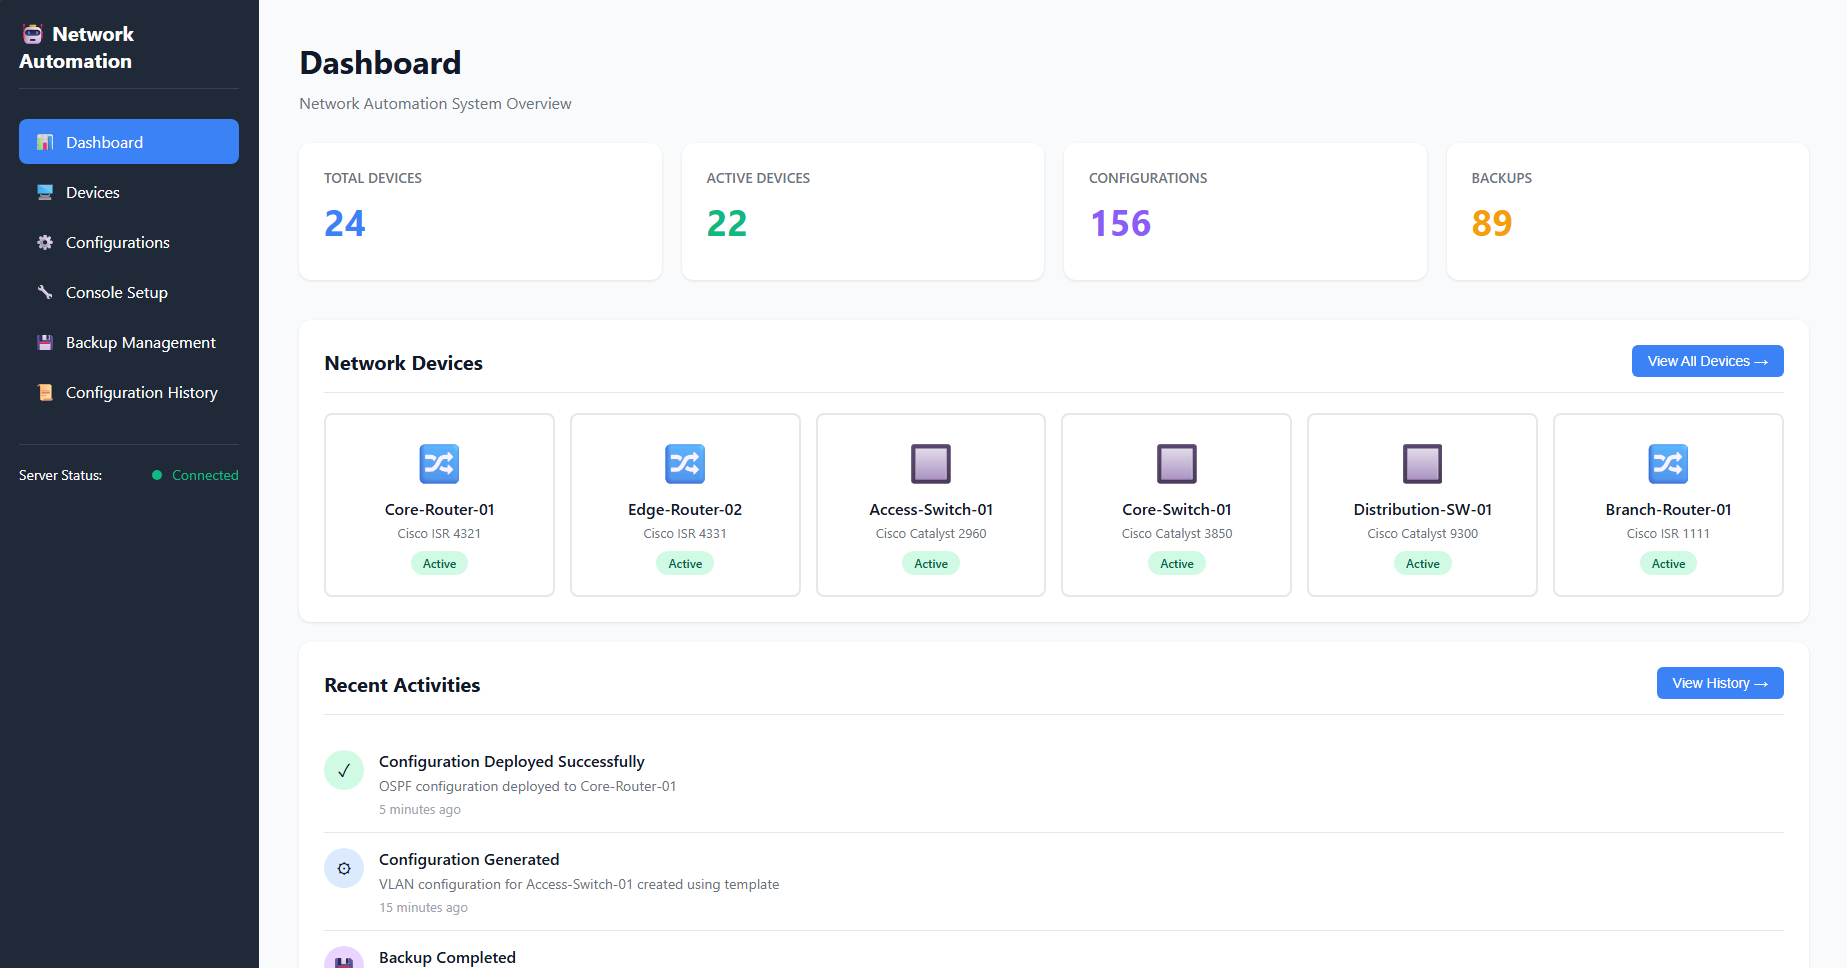
\includegraphics[width=1.0\textwidth]{Image/mockup-1.png}
}
\caption{\fontSixTeen{หน้าจอ Dashboard}}
\label{fig3:Dashboard}
\end{figure}

\hspace*{1.3em} %ย่อหน้า
จากภาพที่ \ref{fig3:Dashboard} หน้า Dashboard ถูกออกแบบมาเพื่อให้ผู้ใช้งานสามารถเห็นภาพรวมของระบบได้อย่างรวดเร็วและชัดเจน
\begin{mycustomitem}
    \item แสดงสถิติภาพรวม
    \item แสดงรายการอุปกรณ์
    \item แสดงกิจกรรมล่าสุด
\end{mycustomitem}
การออกแบบในรูปแบบนี้ช่วยให้ผู้ดูแลระบบสามารถติดตามสถานะของระบบเครือข่ายได้อย่างรวดเร็ว

\begin{figure}[H]
\centering
\adjustbox{frame, width=1.0\textwidth}{%สร้างกรอบของภาพ
    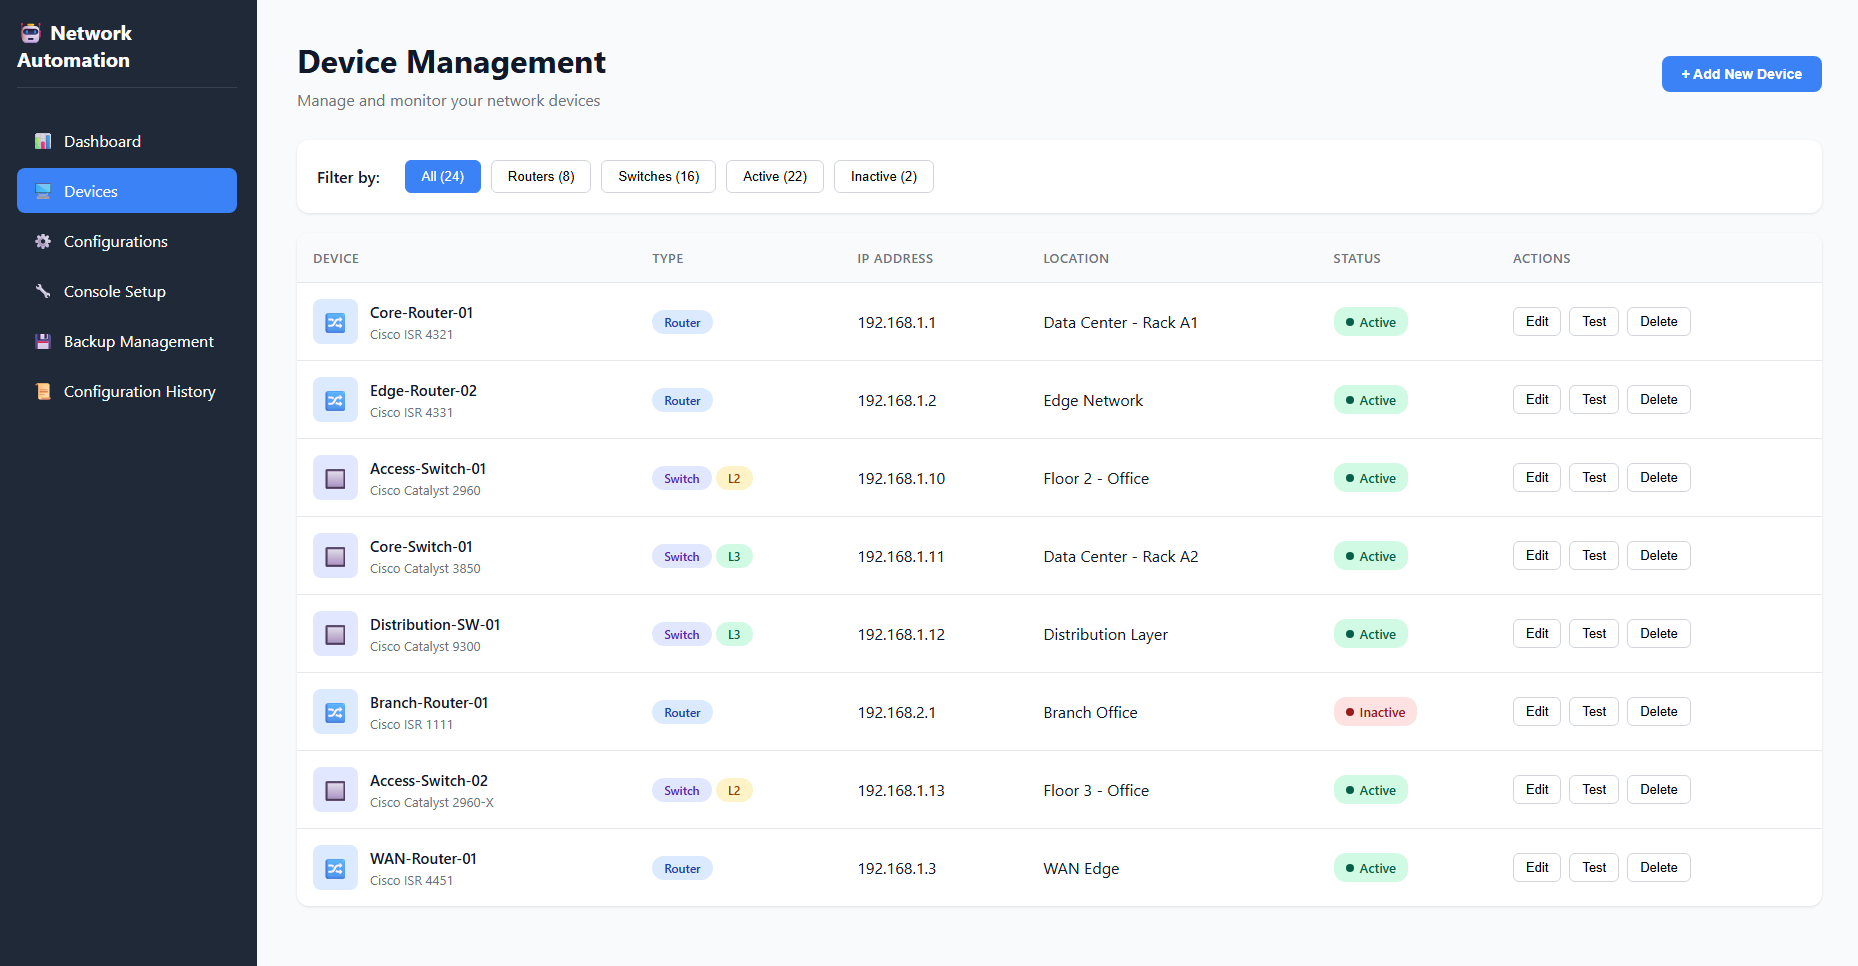
\includegraphics[width=1.0\textwidth]{Image/mockup-2.png}
}
\caption{\fontSixTeen{หน้าจอ Device Management}}
\label{fig3:DeviceManagement}
\end{figure}

\hspace*{1.3em} %ย่อหน้า
จากภาพที่ \ref{fig3:DeviceManagement} หน้า Device Management ถูกออกแบบมาเพื่อให้ผู้ใช้งานสามารถจัดการข้อมูลอุปกรณ์เครือข่ายทั้งหมดในระบบได้อย่างมีประสิทธิภาพ
\begin{mycustomitem}
    \item ปุ่มเพิ่มอุปกรณ์ใหม่
    \item ฟิลเตอร์การค้นหา
    \item ตารางแสดงรายละเอียดอุปกรณ์
\end{mycustomitem}
การออกแบบนี้ช่วยให้ผู้ดูแลระบบสามารถค้นหา ตรวจสอบ และจัดการอุปกรณ์ในระบบได้อย่างรวดเร็วและมีประสิทธิภาพ 

\hspace*{1.3em} %ย่อหน้า

\begin{figure}[H]
\centering
\adjustbox{frame, width=1.0\textwidth}{%สร้างกรอบของภาพ
    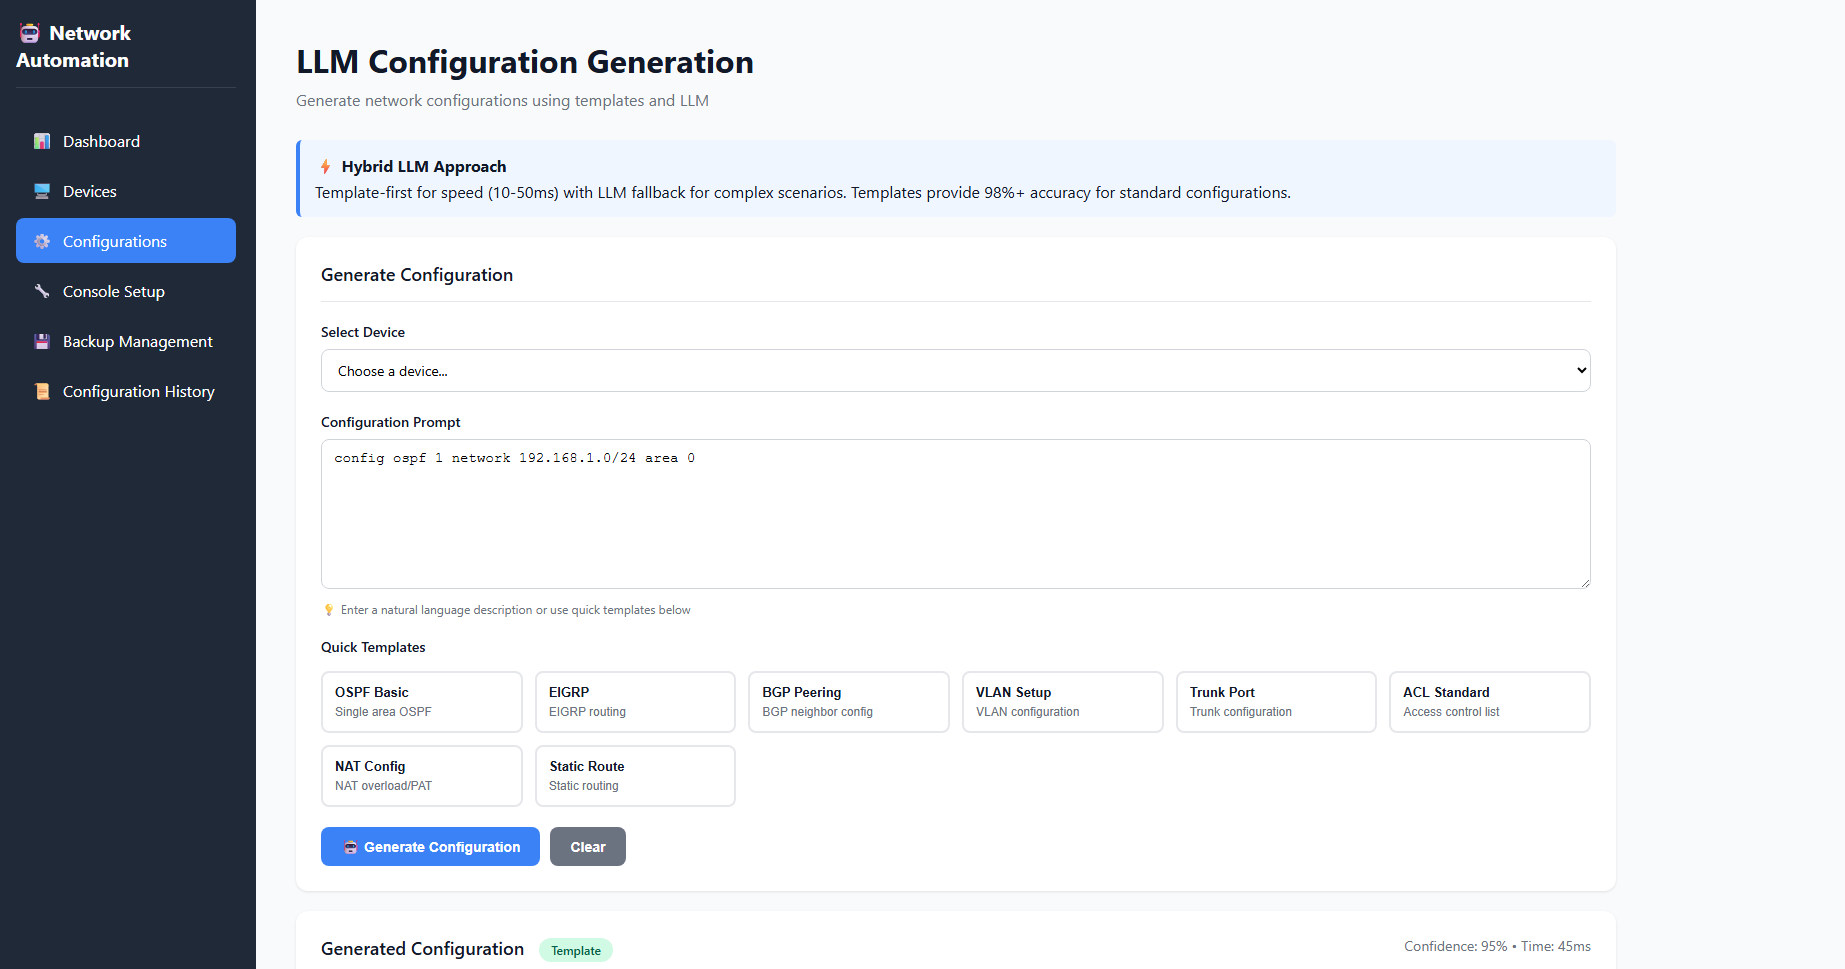
\includegraphics[width=1.0\textwidth]{Image/mockup-3.png}
}
\caption{\fontSixTeen{หน้าจอ LLM Configuration Generation}}
\label{fig3:Config}
\end{figure}

\hspace*{1.3em} %ย่อหน้า
จากภาพที่ \ref{fig3:Config} หน้า LLM Configuration Generation เป็นจุดเด่นหลักของระบบ ซึ่งใช้เทคโนโลยี Large Language Model (LLM) ในการสร้างคำสั่งคอนฟิกสำหรับอุปกรณ์ Cisco โดยอัตโนมัติ 
\begin{mycustomitem}
    \item ส่วนการเลือกอุปกรณ์และป้อนคำสั่ง (รองรับเลือกหลายอุปกรณ์ด้วย Checkbox ในโหมด CLI)
    \item Quick Templates
    \item ส่วนแสดงผลลัพธ์ (แสดงผลแบบ Tab สำหรับแต่ละอุปกรณ์เมื่อเลือกหลายอุปกรณ์)
\end{mycustomitem}
การออกแบบนี้ช่วยลดความซับซ้อนในการเขียนคอนฟิก โดยผู้ใช้เพียงแค่อธิบายสิ่งที่ต้องการเป็นภาษาธรรมชาติ ระบบก็จะสร้างคำสั่งที่ถูกต้องตามมาตรฐาน Cisco ให้อัตโนมัติ และตรวจสอบความถูกต้อง

\hspace*{1.3em} %ย่อหน้า

\begin{figure}[H]
\centering
\adjustbox{frame, width=1.0\textwidth}{%สร้างกรอบของภาพ
    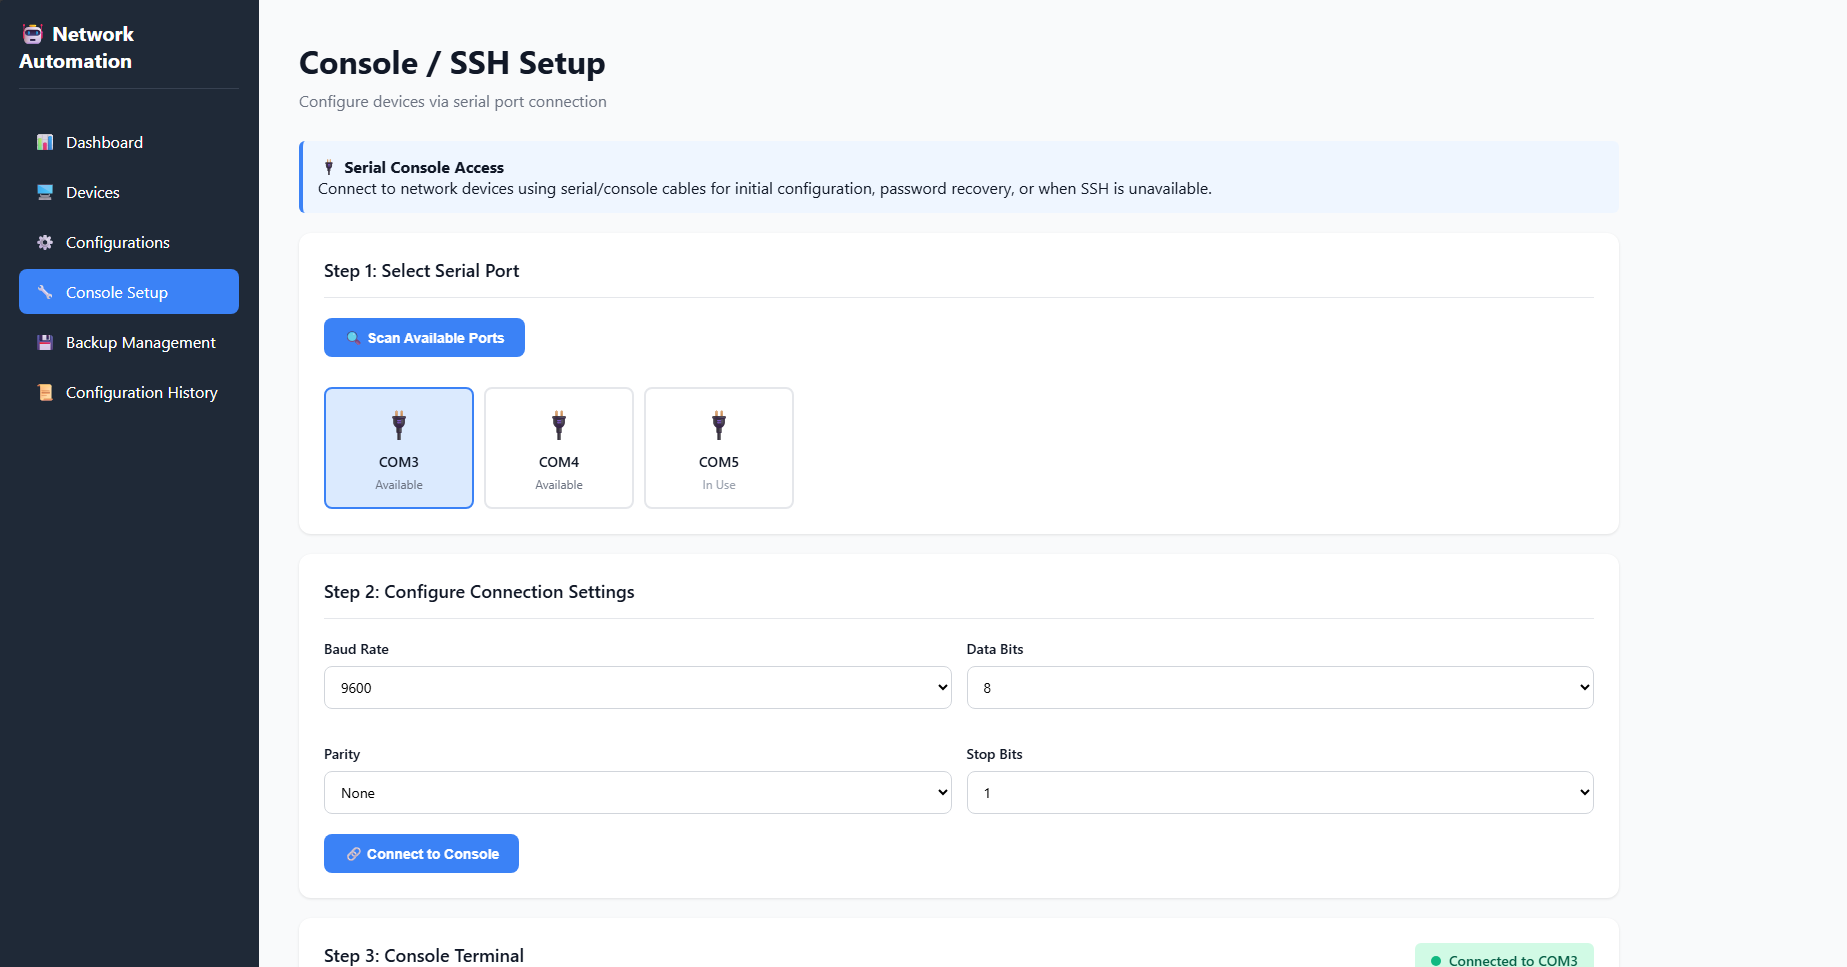
\includegraphics[width=1.0\textwidth]{Image/mockup-4.png}
}
\caption{\fontSixTeen{หน้าจอ Console SSH Setup}}
\label{fig3:ssh1}
\end{figure}

\begin{figure}[H]
\centering
\adjustbox{frame, width=1.0\textwidth}{%สร้างกรอบของภาพ
    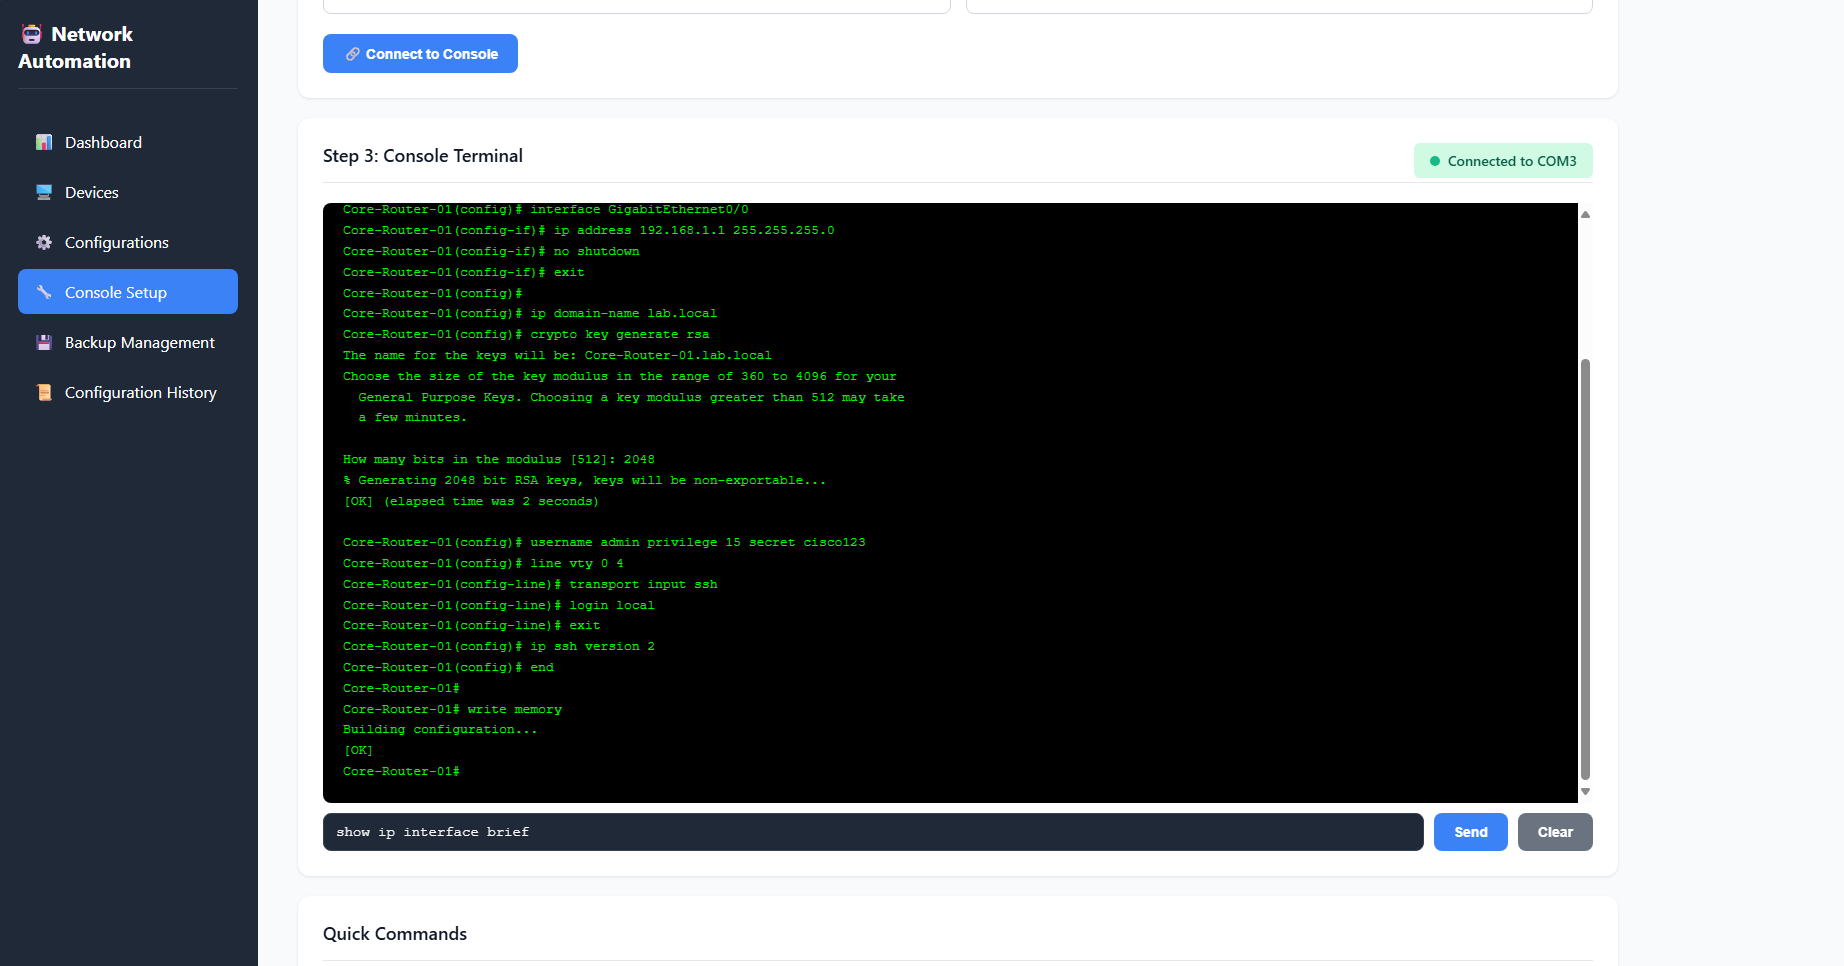
\includegraphics[width=1.0\textwidth]{Image/mockup-5.png}
}
\caption{\fontSixTeen{หน้าจอ Console SSH Setup (ต่อ)}}
\label{fig3:ssh2}
\end{figure}

\begin{figure}[H]
\centering
\adjustbox{frame, width=1.0\textwidth}{%สร้างกรอบของภาพ
    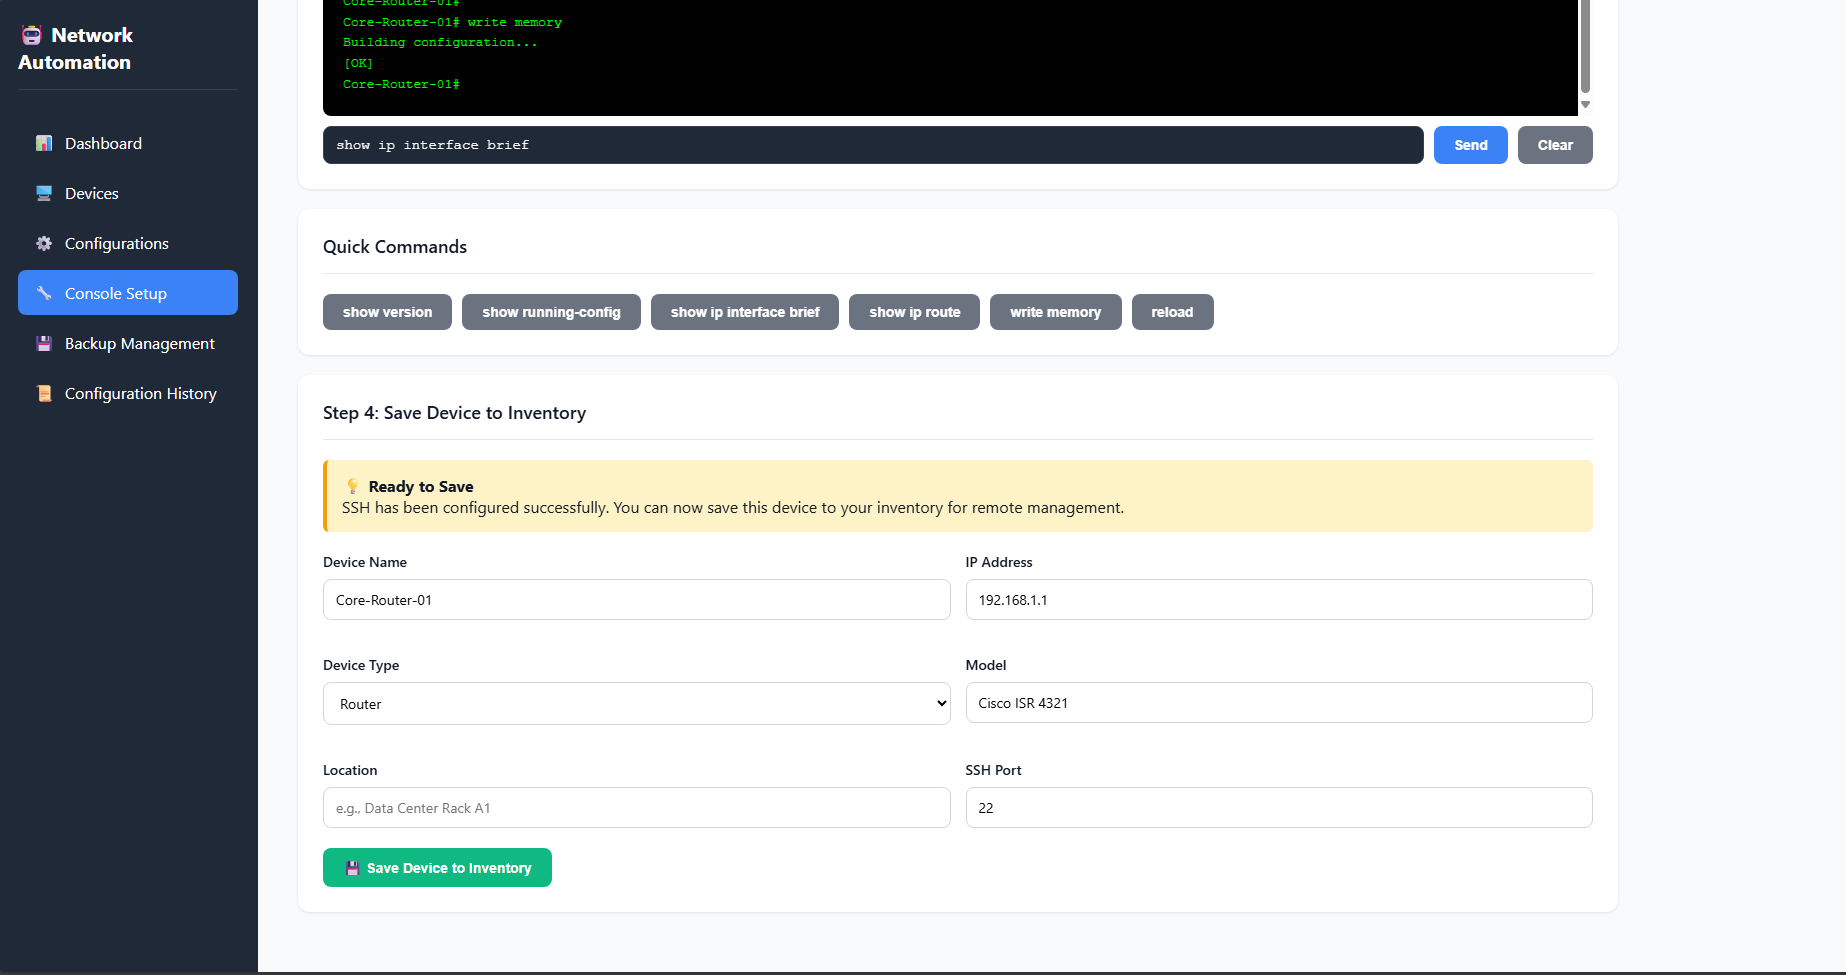
\includegraphics[width=1.0\textwidth]{Image/mockup-6.png}
}
\caption{\fontSixTeen{หน้าจอ Console SSH Setup (ต่อ)}}
\label{fig3:ssh3}
\end{figure}

\hspace*{1.5em}
จากภาพที่ \ref{fig3:ssh1}, \ref{fig3:ssh2} และ \ref{fig3:ssh3} ถูกออกแบบมาเพื่อให้ผู้ใช้งานสามารถเชื่อมต่อกับอุปกรณ์เครือข่ายผ่าน Serial Console Port ได้อย่างสะดวก
\begin{mycustomitem}
    \item Select Port
    \item Configure Connection
    \item Terminal
    \item Save Device
\end{mycustomitem}
การออกแบบนี้ช่วยให้ผู้ใช้สามารถตั้งค่าและเชื่อมต่อกับอุปกรณ์ที่ยังไม่มีการตั้งค่าเครือข่ายได้อย่างถูกต้อง โดยไม่จำเป็นต้องใช้โปรแกรม Terminal แยกต่างหากเพิ่มกำหนดค่า SSH


\begin{figure}[H]
\centering
\adjustbox{frame, width=1.0\textwidth}{%สร้างกรอบของภาพ
    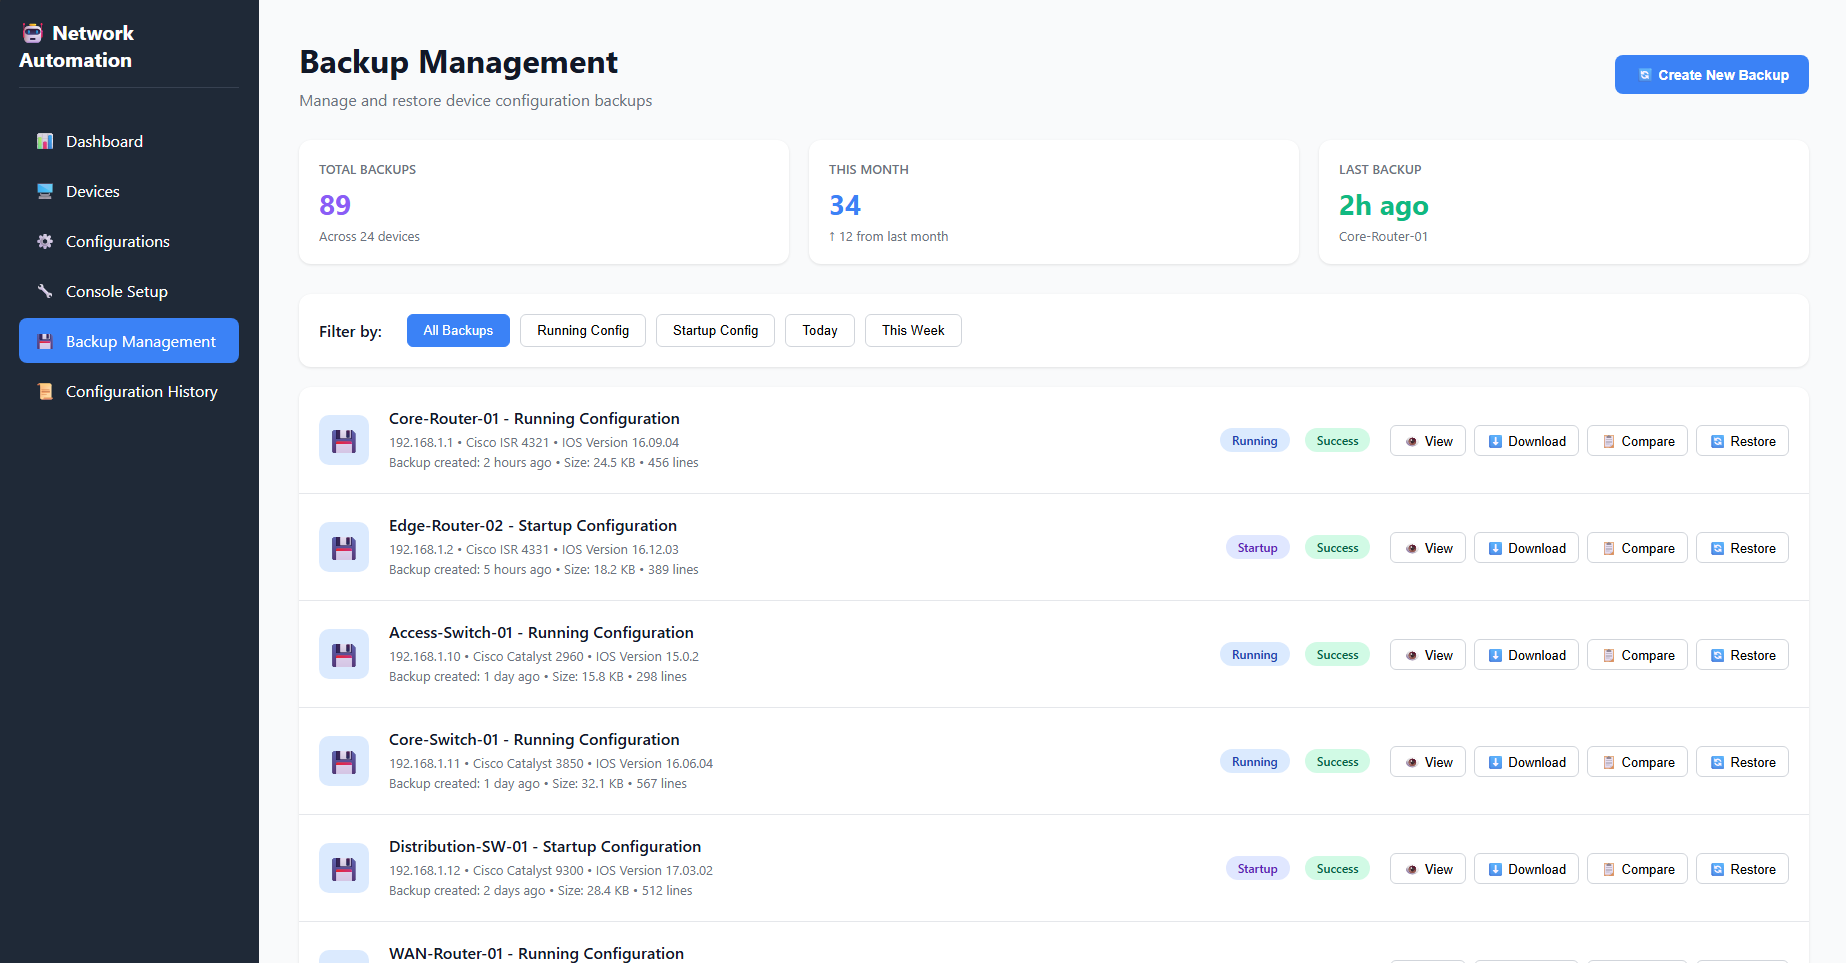
\includegraphics[width=1.0\textwidth]{Image/mockup-7.png}
}
\caption{\fontSixTeen{หน้าจอ Backup Management}}
\label{fig3:backup}
\end{figure}

\hspace*{1.3em} %ย่อหน้า
จากภาพที่ \ref{fig3:backup} หน้า Backup Management ถูกออกแบบมาเพื่อให้ผู้ใช้งานสามารถจัดการสำรองคอนฟิกของอุปกรณ์เครือข่ายได้อย่างมีประสิทธิภาพ
\begin{mycustomitem}
    \item ปุ่มเพิ่ม Backup
    \item ส่วนสรุปข้อมูลการสำรอง
    \item ฟิลเตอร์และการค้นหา
    \item ตารางแสดงรายการสำรอง
    \item Modal สำหรับแสดงตัวอย่างไฟล์
\end{mycustomitem}
การออกแบบนี้ช่วยให้ผู้ดูแลระบบสามารถติดตามและจัดการสำรองคอนฟิกได้อย่างเป็นระบบและสามารถกู้คืนคอนฟิกเมื่อจำเป็นได้อย่างรวดเร็ว

\begin{figure}[H]
\centering
\adjustbox{frame, width=1.0\textwidth}{%สร้างกรอบของภาพ
    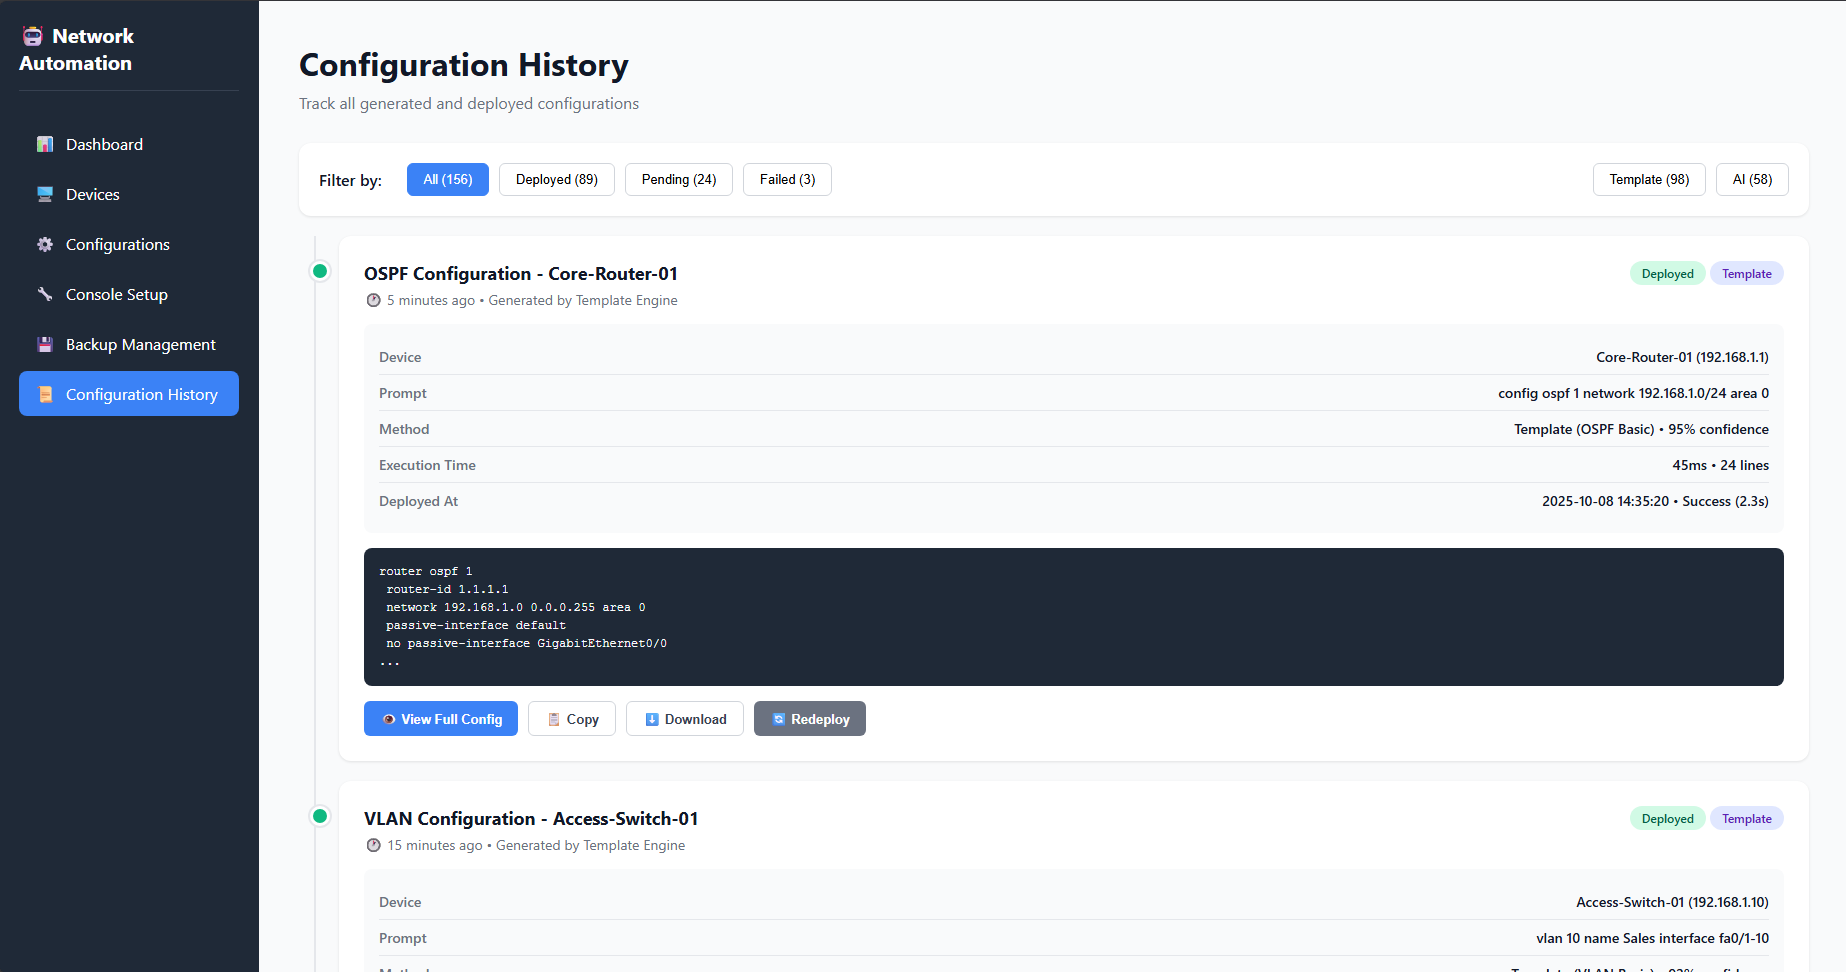
\includegraphics[width=1.0\textwidth]{Image/mockup-8.png}
}
\caption{\fontSixTeen{หน้าจอ Configuration History}}
\label{fig3:history}
\end{figure}

\hspace*{1.3em} %ย่อหน้า
จากภาพที่ \ref{fig3:history} หน้า Configuration History ถูกออกแบบมาเพื่อแสดงบันทึกการเปลี่ยนแปลงคอนฟิกทั้งหมดที่เกิดขึ้นในระบบ ช่วยให้สามารถตรวจสอบและติดตามการเปลี่ยนแปลงได้อย่างละเอียด 
\begin{mycustomitem}
    \item ฟิลเตอร์การแสดงผล
    \item Timeline แสดงประวัติ
    \item Actions
\end{mycustomitem}
การออกแบบในรูปแบบ Timeline นี้ช่วยให้ผู้ดูแลระบบสามารถติดตามการเปลี่ยนแปลงที่เกิดขึ้นกับอุปกรณ์แต่ละเครื่องได้อย่างชัดเจน สามารถตรวจสอบว่าการเปลี่ยนแปลงใดสำเร็จหรือล้มเหลว และสามารถย้อนกลับไปใช้คอนฟิกเก่าได้เมื่อจำเป็น 